% AUTO-GENERATED by scripts/build_single_main_tex.py.
% Edit main.tex, sections/*.tex, or tables/*.tex, then regenerate this file.
% Class/style, bibliography, and figure assets intentionally remain external.
\PassOptionsToPackage{hyperfootnotes=false}{hyperref}
\documentclass[a4paper,fleqn]{cas-dc}

\usepackage[numbers,sort&compress]{natbib}
\usepackage{graphicx}
\graphicspath{{./}{figures/}}
\DeclareGraphicsExtensions{.pdf,.png,.jpg,.jpeg}
\usepackage{amsmath,amssymb}
\usepackage{booktabs}
\usepackage{multirow}
\usepackage{needspace}
\usepackage{placeins}
\usepackage{lastpage}
\usepackage{url}

\begin{document}
\def\lastpage{\pageref{LastPage}}
% cas-common.sty prints an empty ORCID footnote even when no ORCID is supplied.
\RenewDocumentCommand{\printorcid}{}{}
\let\WriteBookmarks\relax
\def\floatpagepagefraction{1}
\def\textpagefraction{.001}

\shorttitle{Category Limits for Few-Shot Certification}
\shortauthors{Thai and Nguyen}

\title[mode = title]{How Many Categories Are Enough? Distribution-Free Certification Limits for Few-Shot Anomaly Thresholds}

\author[1]{Gia Huy Thai}
\ead{23120008@student.hcmus.edu.vn}

\author[2]{Anh Nguyen}
\cormark[1]
\ead{anh.nt@vlu.edu.vn}

\affiliation[1]{organization={University of Science, VNU-HCM},
                city={Ho Chi Minh City},
                country={Vietnam}}

\affiliation[2]{organization={Faculty of Information Technology, Van Lang School of Technology, Van Lang University},
                city={Ho Chi Minh City},
                country={Vietnam}}

\cortext[cor1]{Corresponding author.}

% BEGIN INLINED FILE: sections/abstract.tex
\begin{abstract}
At the nominal false-alarm level $\alpha=0.20$, a target-only leave-one-image-out (LOIO) alarm reaches an empirical false-alarm rate (FAR) of 0.341 on Gaussian-corrupted MVTec at $k=4$, approximately 1.7 times the requested level. This motivates a study-design question: how much source evidence, measured in images or category units, can support threshold certification for a new category? Using a frozen DINOv2 principal component analysis (PCA) residual ranker, we audit 15 MVTec and 12 VisA categories under four corruptions. Target-only rank values have the finite resolution floor $1/(k{+}1)$, yet crossing it does not restore false-alarm stability under shift. We derive a category-count feasibility calculus. Even with zero observed category losses, an optimistic multiplicity-free, deterministic, uniformly valid, distribution-free 95\% upper confidence bound (UCB) requires at least 14, 29, and 59 independent and identically distributed (iid) category draws at $\alpha=0.20$, 0.10, and 0.05. These counts are necessary, not sufficient. Cross-category Reliability Estimation with Source Support (CRESS) separates reference, threshold-proposal, and certification categories. With only three or four certification categories, every target cell evaluated under category-unit certification across 960 frozen gate configurations receives the fail-closed threshold $\tau^\star=0$; the smallest category-level UCB is 0.950, far above the largest tested $\alpha$. Under an idealized iid source-image model, image-unit sensitivity bounds select positive thresholds in 36.7\% to 60.3\% of target cells, but address the selected source mixture rather than marginal risk over a new-category draw. The main contribution is a quantitative feasibility boundary and an estimand-aware protocol for deciding when source evidence can, and cannot, justify a transferable reliability claim.
\end{abstract}
% END INLINED FILE: sections/abstract.tex

% \begin{graphicalabstract}
% 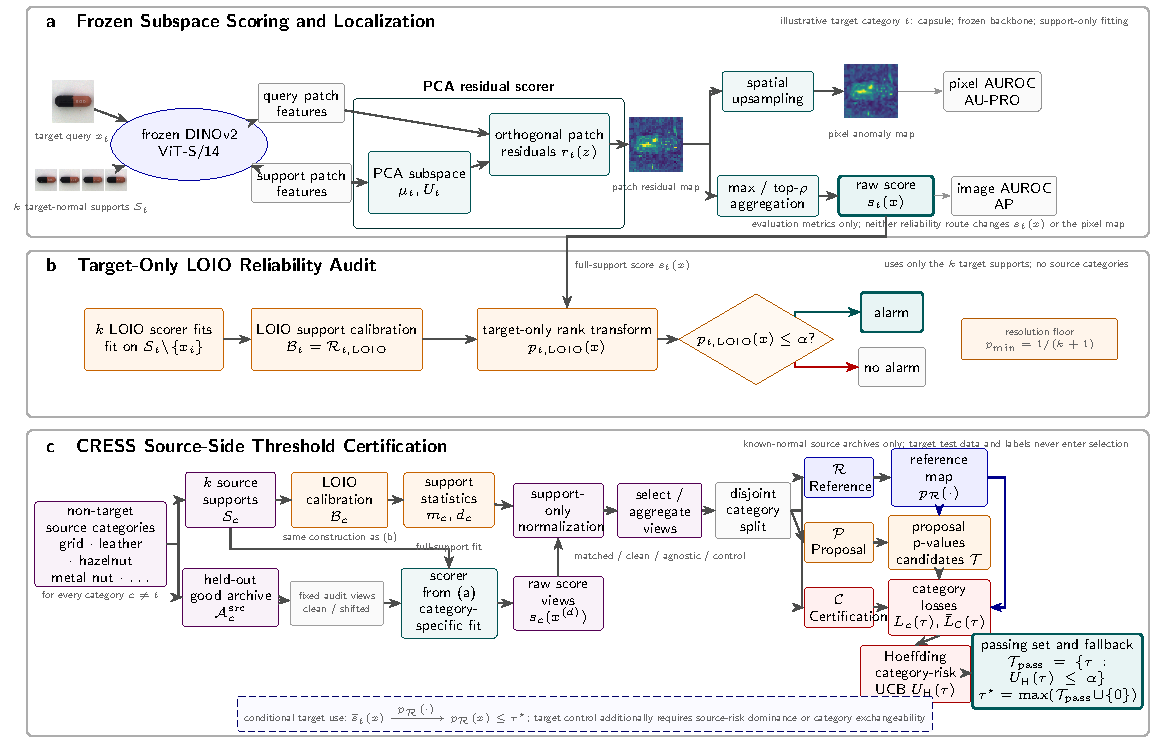
\includegraphics[width=0.86\textwidth]{fig_pipeline}
% \end{graphicalabstract}

% \begin{highlights}
% \item Target-only MVTec false-alarm rate reaches 0.341 under Gaussian noise
% \item Even with no failures, risk 0.20 needs 14 independent same-population categories
% \item All 960 frozen configurations fail closed with only three or four categories
% \item Image-unit bounds target a source mixture, not an unseen category
% \end{highlights}

\begin{keywords}
Industrial anomaly detection \sep Few-shot learning \sep Conformal prediction \sep Distribution-free certification \sep Distribution shift \sep Reliability
\end{keywords}

\maketitle
% CAS writes default PDF metadata during front-matter construction; set the
% final submission metadata afterwards so author separators remain portable.
\hypersetup{
  pdftitle={How Many Categories Are Enough? Distribution-Free Certification Limits for Few-Shot Anomaly Thresholds},
  pdfauthor={Gia Huy Thai and Anh Nguyen},
  pdfsubject={Reliability and certification limits for few-shot industrial anomaly detection},
  pdfkeywords={industrial anomaly detection, few-shot learning, conformal prediction, distribution-free certification, distribution shift, reliability},
  pdfcreator={LaTeX using the Elsevier CAS double-column class}
}

% BEGIN INLINED FILE: sections/introduction.tex
\section{Introduction}\label{sec:introduction}
At the nominal false-alarm level $\alpha=0.20$, the target-only alarm studied in this paper reaches an empirical FAR of 0.341 on Gaussian-corrupted MVTec at $k=4$. This is the largest dataset-level aggregate in the frozen corruption grid and is approximately 1.7 times the requested level. It is not a population-level failure probability: it is a benchmark observation pooled over categories and five support-sampling seeds under one declared synthetic shift. Nevertheless, it exposes an operational gap that ranking metrics alone cannot reveal. A detector may assign defects higher anomaly scores than normal images and obtain a strong area under the receiver operating characteristic curve (AUROC) or average precision (AP), while a fixed score threshold still produces substantially different false-alarm behavior across categories or input conditions.

This gap is particularly consequential in few-shot industrial anomaly detection (AD). A target category commonly provides only $k\in\{1,2,4,8\}$ known-normal support images, whereas anomalous examples are rare, heterogeneous, and unavailable for threshold fitting. Frozen visual foundation models make ranking feasible in this regime: DINOv2~\cite{oquab2024dinov2} patch features support nearest-neighbor (NN) memory banks, as in PatchCore-style methods and AnomalyDINO~\cite{roth2022towards,damm2025anomalydino}, or compact PCA normal subspaces, as in SubspaceAD~\cite{subspacead2026}. These advances do not by themselves specify which alarm threshold has a stable operational meaning.

Two responses are natural. The first is to calibrate on the $k$ target-normal supports. Our target-only route evaluates each support image in a LOIO fit and ranks a test score against the resulting normal scores. This construction is label-free and interpretable, but its rank values occupy only the grid $\{j/(k+1)\}$. Increasing $k$ refines that grid; it does not ensure that support and shifted test scores satisfy the exchangeability conditions needed for false-alarm validity. The empirical FAR of 0.341 is an example of this distinction: the operating level is attainable, yet the shifted-normal rank distribution is anti-conservative relative to the exchangeable reference.

The second response is to borrow normal evidence from non-target source categories. A larger source archive offers finer empirical ranks and can propose thresholds below the target-only grid. It also changes the statistical question. Independent image draws from a declared source mixture can estimate risk for that mixture, whereas a guarantee intended for a previously unseen category depends on iid category units from a declared meta-population. Repeated images, corruption views, or support seeds do not create new category units. The central question of this paper is therefore:

\begin{quote}
How much source evidence, measured in which statistical unit, is needed to certify an anomaly threshold for a new category?
\end{quote}

We answer this question at three levels. First, for any deterministic, uniformly valid, distribution-free 95\% UCB based only on iid category losses, an all-zero sample cannot certify $\alpha=0.20$, 0.10, or 0.05 with fewer than 14, 29, or 59 categories, respectively, even without multiplicity. These are optimistic impossibility-side limits, not sufficient sample sizes for the implemented procedure. Under the frozen simultaneous allocation, the corresponding lower limits are at least 22, 46, and 94 for one candidate, while the declared Hoeffding rule requires 60, 240, and 958. Second, we audit target-only normal rank values under four controlled corruptions and show that crossing the finite resolution floor does not imply a stable FAR\@. Third, we use CRESS to separate source categories into disjoint reference, threshold-proposal, and certification roles and test whether the available archive reaches the predicted feasibility boundary.

CRESS is a source-assisted thresholding and audit protocol, not a new anomaly ranker. The inherited ranking substrate is a frozen DINOv2 PCA residual. The reference categories define a source-reference rank map, the proposal categories define a finite candidate set, and the certification categories evaluate fixed candidates with a family-adjusted UCB\@. The protocol returns the largest passing threshold or the fail-closed value zero. Source-risk dominance can transfer the bound to a particular target category. An iid category-sampling model supports only a marginal bound averaged over a new-category draw, not category-conditional control for every realized target. Normalization and source pooling establish neither condition.

The strict audit contains only three certification categories in VisA cells and four in MVTec and transfer cells. This shortage is not solely a consequence of the frozen $0.50/0.25/0.25$ split. The eligible source pools contain 11, 14, or 15 categories, so keeping the reference and proposal roles nonempty leaves at most 9, 12, or 13 certification categories, all below the optimistic 14-category limit at $\alpha=0.20$. Accordingly, category-unit certification assigns $\tau^\star=0$ to every target cell across the 960 frozen configurations. This is not 960 independent failures, nor a compute or optimization failure. The configurations span jobs, source-view modes, support sizes, nominal levels, and conditions, but share the same category-count obstruction. Their value is to show that the fail-closed outcome persists throughout the declared grid in the regime where the analytic calculation predicts non-feasibility. By contrast, under the idealized iid source-image model, image-unit analyses have 72 to 191 units per cell and select positive thresholds in 36.7\% to 60.3\% of target cells, depending on the source-to-target job. This contrast is not a stronger-versus-weaker version of one certificate: the two analyses target different risks. The same source archive is statistically large when counted in images but insufficient when the deployment claim concerns marginal risk for a new-category draw.

The paper makes three contributions:
\begin{itemize}
    \item \textbf{A category-count feasibility calculus.} We derive the Hoeffding-specific requirement and a broader all-zero lower bound for deterministic uniformly valid distribution-free category-risk upper bounds. The resulting calculations quantify the minimum budget of iid category draws implied by the requested risk and confidence levels and serve as a study-design tool rather than a post hoc explanation alone.
    \item \textbf{An operational shift audit.} Across 15 MVTec and 12 VisA categories, the target-only analysis distinguishes unattainable nominal levels from attainable but unstable operating points. The largest dataset-level aggregate FAR is 0.341 on Gaussian-corrupted MVTec at $k=4$ and $\alpha=0.20$; VisA is conservative in the corresponding cells, showing that the shift effect is dataset-dependent rather than universal.
    \item \textbf{An estimand-aware source protocol.} CRESS separates reference, proposal, and certification categories, retains zero fallbacks, and reports image-mixture and category-level conclusions without substituting one for the other. The frozen strict audit verifies the predicted category shortage within datasets and for transfer from MVTec to VisA and the Metal Parts Defect Dataset (MPDD); direct pooling and compact-ranker results are reported only as supporting empirical context.
\end{itemize}

Figure~\ref{fig:certificate-feasibility} previews the central design calculation. The black curve is the optimistic multiplicity-free floor for deterministic uniformly valid distribution-free bounds in the scope of Proposition~3; the blue and orange curves add the frozen family allocation and the declared Hoeffding rule in their most favorable one-candidate case. A positive certificate is infeasible within the corresponding rule class whenever its curve remains above the requested $\alpha$. The shaded region marks the three or four certification categories available in the strict audit; Table~\ref{tab:certificate-feasibility} later reports the exact candidate-family calculations.

\begin{figure*}[pos=t]
    \centering
    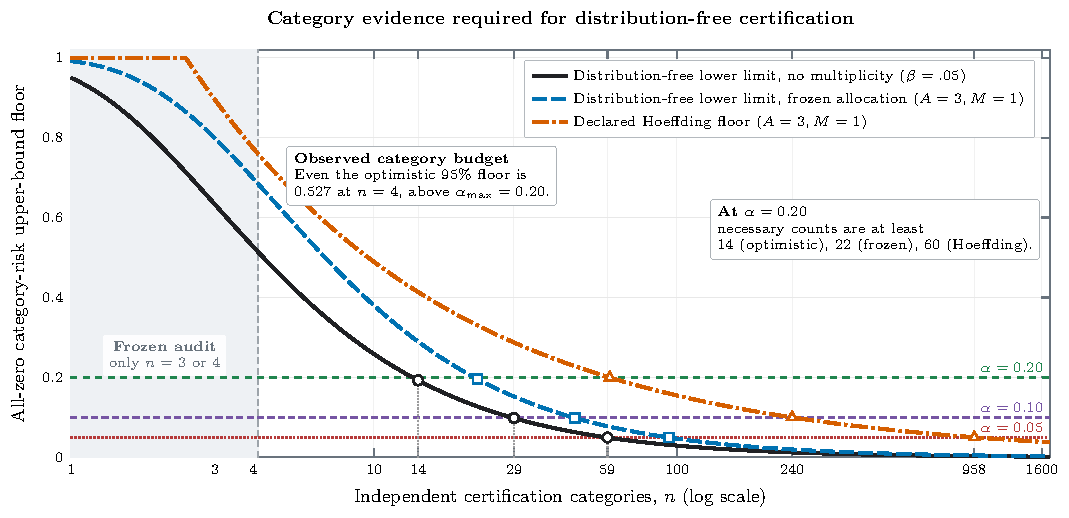
\includegraphics[width=0.97\linewidth]{fig_certificate_feasibility}
    \caption{Analytic category-count feasibility after observing zero loss in every certification category. The black curve is the multiplicity-free lower bound $1-0.05^{1/n}$ for deterministic uniformly valid distribution-free procedures in Proposition~3. The blue curve applies the frozen allocation $\beta=\delta/(2AM)$ with $\delta=0.05$, $A=3$ reported levels, and the favorable one-candidate case $M=1$; the orange curve is the corresponding Hoeffding floor. Horizontal lines mark the requested risk levels, and the shaded region marks the three or four distinct certification categories available in the frozen audit; interpreting them as iid units is a modeling assumption. The black circular crossings at the 14, 29, and 59 axis ticks mark optimistic necessary counts without multiplicity, not sufficient sample sizes for CRESS\@. A curve above a requested $\alpha$ rules out a positive threshold only within its stated procedure class, even under all-zero observed category loss.}
    \label{fig:certificate-feasibility}
\end{figure*}

The remainder of the paper is organized as follows. Section~\ref{sec:related} positions the study against few-shot detectors, calibration, and conformal risk control. Section~\ref{sec:method} defines the inherited scorer, target-only route, source construction, CRESS protocol, and certificate scope. Section~\ref{sec:experiments} specifies the frozen datasets, statistical units, partitions, and claim rules. Section~\ref{sec:results} proceeds from the shift audit to category-count feasibility and strict CRESS, followed by the supporting ranking and storage analysis. Sections~\ref{sec:limitations} and~\ref{sec:conclusion} state the boundaries and implications.
% END INLINED FILE: sections/introduction.tex
% BEGIN INLINED FILE: sections/related_work.tex
\section{Related Work}\label{sec:related}
\subsection{Few-Shot Industrial AD}
Classical industrial AD typically assumed access to normal-only training data and identified deviations at test time. Patch distribution, self-supervised, and reconstruction-discriminative approaches such as PaDiM, CutPaste, and DRAEM provided important context for this literature~\cite{padim2021,cutpaste2021,draem2021}. PatchCore~\cite{roth2022towards} established memory-bank patch retrieval as a robust baseline by storing representative normal features and scoring test patches using NN distance. AnomalyDINO~\cite{damm2025anomalydino} extended this paradigm to few-shot inspection with frozen DINOv2 representations. Subsequent work introduced registration-based adaptation (RegAD~\cite{regad2022}), graph-structured memory (GraphCore~\cite{graphcore2023}), and fast feature reconstruction (FastRecon~\cite{fastrecon2023}). Vision-language methods included WinCLIP~\cite{winclip2023}, CLIP-SAM collaboration~\cite{clipsam2025}, and cross-modal prompt regularization~\cite{uniadprompt2026}; InCTRL introduced in-context residual learning~\cite{inctrl2024}. These methods were effective rankers, but their raw score scales did not by construction carry a certified FAR interpretation. Calibration under distribution shift was also known to degrade for deep models generally~\cite{ovadia2019trust}. Our work is complementary: it does not compete on ranking but instead examines how few-shot detectors should expose decision reliability.

\subsection{Frozen-Feature Subspace Detectors}
Subspace approaches replaced explicit patch retrieval with a compact normal subspace. SubspaceAD~\cite{subspacead2026} demonstrated that frozen DINOv2 patch features and PCA or subspace residuals were already effective for few-shot anomaly ranking, establishing the ranking mechanism as prior art. Our contribution begins after the residual is computed and examines the reliability claims that a low-storage subspace detector can support under few-shot and distribution-shift conditions.

\subsection{Calibration and Decision Reliability in Few-Shot AD}
Calibration measured agreement between predicted confidence and empirical correctness~\cite{platt1999,guo2017calibration}. Standard post-hoc methods included Platt scaling and temperature scaling~\cite{platt1999,guo2017calibration}. Histogram binning and isotonic regression provided nonparametric alternatives~\cite{zadrozny2001obtaining,zadrozny2002transforming}. Sparse labels, open-ended anomaly types, and category-dependent scores made this objective especially difficult in AD\@. Prior reliability analyses of few-shot AD based on DINOv2 also documented calibration and perturbation sensitivity~\cite{khan2025calibration}. These findings motivated our separation of ranking quality from an operational question: whether a declared alarm rule maintains its requested false-alarm behavior under a specified shift. A calibrated probability summary alone would not constitute such a risk guarantee.

\subsection{Conformal Prediction and Risk-Controlled Calibration}
Conformal prediction transformed nonconformity scores into p-values under exchangeability assumptions~\cite{vovk2005,shafer2008tutorial,angelopoulos2021gentle}. This approach was particularly suitable for normal-only few-shot AD because normal support images could define a reference distribution without requiring real anomalies. Conformal AD was already well established: leave-one-out, bootstrap, and cross-conformal anomaly detectors had been directly analyzed~\cite{hennhofer2024loio}; weighted conformal detection in low-data regimes had examined resolution and effective-sample-size effects~\cite{hennhofer2026weighted}; general nonconformity toolkits had been developed~\cite{hennhofer2026nonconform}; and few-shot conformal prediction with auxiliary tasks had addressed small target calibration sets~\cite{fisch2021fewshot}. Conformal AD, LOIO calibration, auxiliary-task transfer, and weighted conformal p-values were therefore established mechanisms.

Risk-controlling calibration also preceded our work. Learn then Test cast finite-sample calibration as a multiple-testing problem over candidate configurations~\cite{angelopoulos2021learntest}, while conformal risk control selected a parameter to control the expectation of a monotone loss~\cite{angelopoulos2024crc}. In AD, PAC-Wrap provided semi-supervised probably approximately correct (PAC) bounds for false-positive and false-negative rates around a base detector~\cite{li2022pacwrap}. These works established the general principles of candidate testing, held-out risk assessment, and one-sided error bounds; we do not claim those statistical primitives as new. CRESS instead instantiates them for normal-only cross-category thresholding by assigning disjoint source categories to reference, proposal, and certification roles, distinguishing selected-mixture image risk from marginal new-category risk, and auditing whether the available category count can support a nonzero threshold under the declared iid model.

Structure-aware conformal adaptation had also been studied outside AD\@. Lam and Anh proposed Heterophily-Aware Diffused Conformal Prediction (HeAD-CP), which adapted graph-score diffusion using label-free local homophily estimates and showed that uniform diffusion could impair prediction-set efficiency on heterophilic graphs while preserving marginal coverage~\cite{lam2026headcp}. This result supported the broader need to audit reliability transformations under structural shift, but its setting concerned graph neural network (GNN) node-classification sets rather than few-shot industrial anomaly alarms or cross-category source certification.

The deterministic source-view choices were conceptually informed by the shared-versus-specialized selection motif in Shape-Adapting Gated Experts (SAGE)~\cite{Thai_2026_CVPR}. That work concerned learned expert selection rather than certification of anomaly thresholds. CRESS uses no learned expert gate: its source-view modes are predeclared protocol choices, and its reference, proposal, and certification partitions have disjoint statistical roles. The citation therefore records design inspiration without attributing CRESS validity or novelty to the SAGE architecture.

The present contribution begins at the independent-category requirement of a simultaneous source certificate, with the target-only grid $1/(k{+}1)$ serving as a motivating finite-resolution constraint. We specialize established confidence tools into Hoeffding-specific and distribution-free all-zero category-budget calculations, empirically audit corruption-shift deviations, and evaluate source-assisted candidate thresholds without target anomaly labels. CRESS does not introduce a new nonconformity score or generic confidence bound; it specifies how source categories are separated into reference, proposal, and certification roles and audits whether the resulting source certificate can be nonvacuous at the available category count.
% END INLINED FILE: sections/related_work.tex
% BEGIN INLINED FILE: sections/method.tex
\section{Method}\label{sec:method}
\subsection{Problem Setup}
For each target category $c$, we observe a support set $\mathcal{S}_c=\{x_i\}_{i=1}^{k}$ containing only normal images. Target test images may be normal or anomalous, but their labels are reserved exclusively for evaluation and do not enter detector fitting, threshold proposal, or certification. Other categories may additionally provide a declared source-normal archive. The framework produces a fixed raw anomaly score $s_c(x)$ and optional pixel map, a target-only reliability value $p_{\mathrm{LOIO}}(x)$ when LOIO calibration is available, and, for the source-assisted route, a threshold $\tau^\star$ accompanied by a source-domain certificate. Figures~\ref{fig:target-pipeline} and~\ref{fig:cress-pipeline} separate the inherited ranking substrate, the target-only route, and the source-assisted route.

The statistical unit is fixed before threshold evaluation. Under the idealized iid image model, an image-unit analysis gives equal weight to each retained source image and therefore targets the mean alarm loss for a draw from the induced source-image mixture, whose category weights are proportional to retained image counts. A category-unit analysis first averages alarms within each source category, gives equal weight to each certification category, and then targets the expected archive-level loss of a new draw from the declared source-category meta-population. Here a category unit comprises the category, its support-set construction, and its predeclared held-out normal-view sampling mechanism. Equating this expectation with the alarm probability of a fresh normal image additionally requires those within-category views to be representative of the declared deployment distribution. Independent category units are still required; additional images, support seeds, or corruption views within an existing category do not increase their number. Neither source estimand is automatically the target-category risk. That transfer requires the additional condition stated at the end of this section.

\subsection{Frozen Patch Features and Subspace Ranking}
We extract patch features with a frozen DINOv2 small Vision Transformer using $14\times14$ patches (ViT-S/14). Each RGB image is resized directly to $518\times518$ pixels and normalized with the ImageNet channel mean and standard deviation. The normalized patch-token output contains a $37\times37$ grid of $d=384$ vectors. Let $z_{ij}\in\mathbb{R}^{d}$ denote patch $j$ from image $i$. A PCA subspace is fit on all target-support patches. With support mean $\mu_c$ and retained principal directions $U_c\in\mathbb{R}^{d\times m}$, the patch residual is
\begin{equation}\label{eq:residual}
    r_c(z)=\left\|(z-\mu_c)-U_cU_c^{\top}(z-\mu_c)\right\|_2.
\end{equation}
The patch residuals form an anomaly map. For the conformal protocols, write the $N=1369$ residuals in descending order as $r_{c,(1)}(x)\geq\cdots\geq r_{c,(N)}(x)$ and define the image-level ranking score by
\begin{equation}\label{eq:score}
    s_c(x)=\frac{1}{q}\sum_{j=1}^{q}r_{c,(j)}(x),
    \qquad q=\lceil0.01N\rceil=14.
\end{equation}
This top-$1\%$ mean is a smoothed maximum. The clean accuracy-storage benchmark instead uses the patch maximum ($q=1$). AUROC and AP are always computed from the fixed score $s_c(x)$ within a declared protocol; none of the subsequent reliability transformations changes that score or its ranking. Certification in this study concerns image alarms, not pixel-map thresholds.

\subsection{Target-Only LOIO Reliability}
For $k\geq2$, the target-only route constructs normal calibration residuals by LOIO support splitting. For each support image $x_i$, a subspace is fit on $\mathcal{S}_c\setminus\{x_i\}$, and the held-out image receives the score $s_{c,-i}(x_i)$. The resulting set
\begin{equation}\label{eq:rloio}
    \mathcal{R}_{c,\mathrm{LOIO}}
    =\{s_{c,-i}(x_i):x_i\in\mathcal{S}_c\}
\end{equation}
serves as target-normal nonconformity evidence. A test image, scored using the subspace fit on all $k$ supports, receives the conformal-form rank value
\begin{equation}\label{eq:loio}
    p_{c,\mathrm{LOIO}}(x)
    =\frac{1+\sum_{r\in\mathcal{R}_{c,\mathrm{LOIO}}}
    \mathbf{1}\{r\geq s_c(x)\}}
    {1+|\mathcal{R}_{c,\mathrm{LOIO}}|}.
\end{equation}
We retain the conventional $p$ notation but call Eq.~\eqref{eq:loio} a rank value unless its validity conditions are invoked. It measures extremeness relative to held-out support normals; neither it nor $1-p_{c,\mathrm{LOIO}}(x)$ is a supervised anomaly posterior.

The construction is asymmetric: each calibration score uses $k-1$ support images, whereas the test score uses all $k$. Equation~\eqref{eq:loio} is therefore a LOIO approximation in the spirit of cross-conformal inference~\cite{vovk2005,barber2021jackknife,hennhofer2024loio}, not a split-conformal p-value with an automatic finite-sample guarantee~\cite{bates2023testing,laxhammar2015inductive}. A matched-LOIO audit scores held-out support and test images under the same fold-specific subspaces and is reported as a sensitivity analysis. We retain the declared construction and audit its normal rank values empirically rather than assuming exchangeability.

\begin{figure*}[t]
\centering
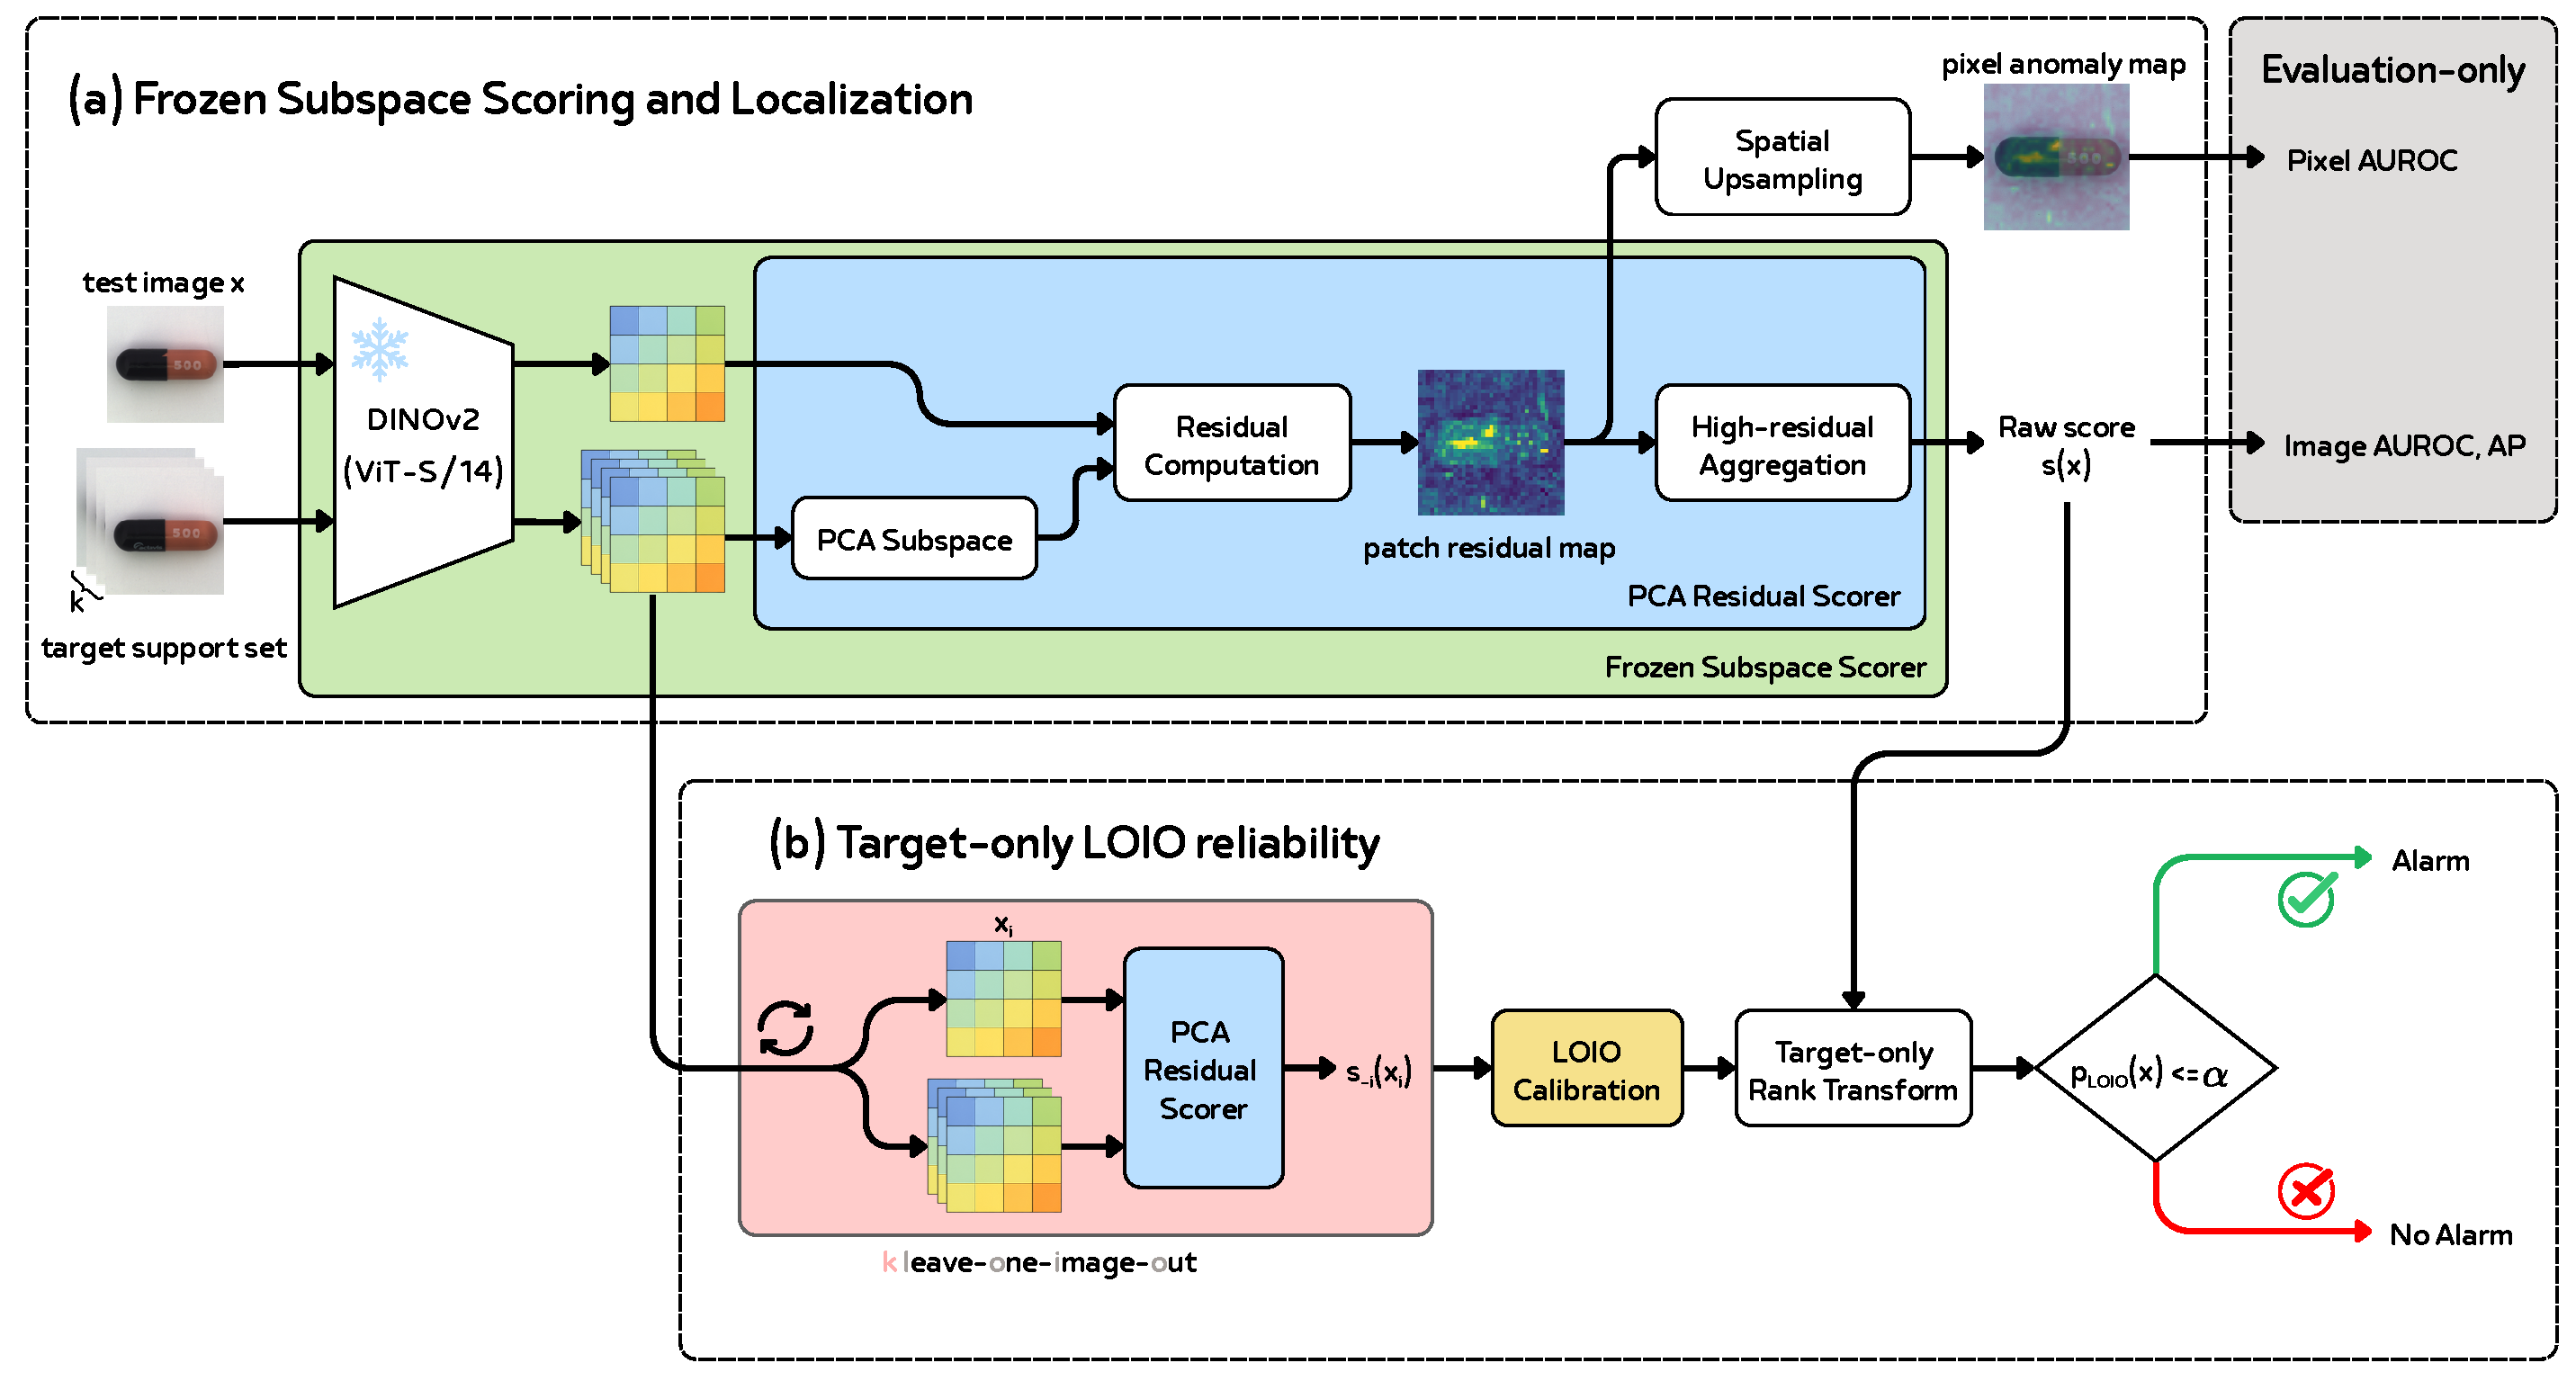
\includegraphics[width=0.98\textwidth]{fig_target_pipeline}
\caption{Target-side scoring and reliability routes. Panel (a) uses frozen DINOv2 patch features and a support-fitted PCA residual scorer to produce the fixed image-ranking score and an optional pixel anomaly map. The metric boxes are evaluation-only; the pixel map is an inherited output, not a certification target or a localization claim of this study. Panel (b) reuses the scorer in LOIO folds to form target-normal calibration scores and the target-only rank value $p_{c,\mathrm{LOIO}}(x)$. Because calibration scores use $k-1$ supports whereas the test score uses all $k$, this rank transform is audited rather than presumed to have automatic finite-sample validity. Its smallest attainable value is $1/(k+1)$, and the alarm rule does not alter the underlying ranking score.}
\label{fig:target-pipeline}
\end{figure*}

\subsection{Target-Only Resolution}
\noindent\textbf{Remark 1 (attainable-alpha floor).} For any finite calibration scores $r_1,\ldots,r_k$, a rank value of the form in Eq.~\eqref{eq:loio} belongs to $\{j/(k{+}1):j=1,\ldots,k{+}1\}$. Hence the alarm $\mathbf{1}\{p(x)\leq\alpha\}$ is identically zero for $\alpha<1/(k{+}1)$.

\noindent\emph{Proof.} The exceedance count is an integer from 0 to $k$. Adding one and dividing by $k+1$ gives the stated grid and lower bound. No exchangeability assumption is needed for this algebraic claim. \hfill$\square$

For $k=4$, the floor is $0.2$; for $k=8$, it is $1/9\approx0.111$. The attainable-alpha analysis reports, for each nominal $\alpha$, the largest attainable grid point not exceeding $\alpha$ and the corresponding empirical FAR\@. The floor is a standard finite-rank resolution property~\cite{hennhofer2026weighted}, not an algorithmic innovation or evidence that the underlying ranker cannot separate anomalies. Randomization can smooth this deterministic grid under the relevant exchangeability assumptions, but it cannot by itself repair support-to-test shift.

\subsection{Source Archive Preparation}\label{sec:cress-source-construction}
CRESS uses known-normal images from categories other than the target. For every target or source category $c$, let $\mathcal{B}_c$ denote its support-only calibration residuals. For $k\geq2$, $\mathcal{B}_c=\mathcal{R}_{c,\mathrm{LOIO}}$. Because LOIO is undefined with one support image, the declared $k=1$ stress test uses one patch-split support calibration residual instead. We summarize $\mathcal B_c$ by its median and median absolute deviation (MAD):
\begin{equation}\label{eq:cress-normalization}
\begin{aligned}
    m_c &= \operatorname{median}(\mathcal{B}_c),\\
    d_c &= \operatorname{MAD}(\mathcal{B}_c),\\
    \widetilde{s}_c(x) &= \frac{s_c(x)-m_c}{\max(d_c,\varepsilon)}.
\end{aligned}
\end{equation}
Here $\varepsilon=10^{-6}$ is fixed before evaluation. This support-only normalization makes cross-category score scales more comparable; it does not establish equality or exchangeability of their distributions. In particular, the single $k=1$ calibration residual has zero MAD, so the denominator is set by the $\varepsilon$ floor; those cells are interpreted as stress tests rather than ordinary LOIO calibration.

The normalized source score views are then selected without inspecting target labels or target scores. Matched-condition mode selects the source view with the declared target condition and therefore requires condition metadata. Clean-source mode always selects clean source normals. Condition-agnostic mode takes, for each base source image, the median normalized score over all available condition views so that repeated corruptions are not counted as independent observations. Deterministic mismatched-condition routing uses the lexicographic successor of the target condition, with wraparound, solely as a negative control. Thus normalization precedes source-view selection or aggregation in the implemented protocol. Only the resulting scalar score archive and category identities are needed downstream; source patch features do not enter certification.

For a fixed target and support seed, the eligible source categories are split before candidate construction into disjoint reference, proposal, and certification sets $\mathcal{R}$, $\mathcal{P}$, and $\mathcal{C}$. The primary allocation is $0.50/0.25/0.25$: integer counts use the largest fractional remainders, with equal remainders resolved toward certification, while keeping every partition nonempty. The category permutation is generated from a hash of the target-category identity and seed, is held fixed across conditions and $k$, and never depends on observed scores, target outcomes, or certification losses. All score views from one category remain in the same partition.

\subsection{Nested CRESS Threshold Selection}\label{sec:cress-threshold-selection}
Let $\mathcal{Z}_{\mathcal{R}}$ be the pooled normalized scores from the selected reference-category views. The reference categories define the source-reference rank map
\begin{equation}\label{eq:cress-source-pvalue}
    p_{\mathcal{R}}(x)
    =\frac{1+\sum_{r\in\mathcal{Z}_{\mathcal{R}}}
    \mathbf{1}\{r\geq\widetilde{s}_c(x)\}}
    {1+|\mathcal{Z}_{\mathcal{R}}|}.
\end{equation}
We use the term \emph{source-reference map} deliberately: Eq.~\eqref{eq:cress-source-pvalue} is an empirical rank transformation on the source archive, and cross-category conformal validity is not presumed. Its finer grid arises from the larger reference-score pool rather than from the $k$ target supports.

Applying the reference map to the proposal categories produces the proposal rank values $\{p_{\mathcal R}(x):x\in\mathcal P\}$. Their distinct values generate an ordered candidate set $\mathcal{T}$. Its realized size is $M=|\mathcal T|$; if it would exceed $M_{\max}=20$, we retain a deterministic evenly spaced subset. Certification data influence neither $\mathcal T$ nor $M$. The same reference map is then applied to every certification image. Given $\tau\in\mathcal T$, its image-unit loss is
\begin{equation}\label{eq:cress-image-loss}
    L_x(\tau)=\mathbf{1}\{p_{\mathcal{R}}(x)\leq\tau\}.
\end{equation}
All certification images are declared normal, so an alarm is a false alarm. For a certification category $c$, the category-unit loss is
\begin{equation}\label{eq:cress-category-loss}
    L_c(\tau)=\frac{1}{n_c}\sum_{x\in c}L_x(\tau)\in[0,1].
\end{equation}
Under iid image sampling, the image unit targets mean loss for the declared source-image mixture. The category unit instead targets expected archive-average loss for a complete category unit drawn iid from the declared meta-population. Treating $L_c(\tau)$ as one bounded unit allows arbitrary dependence among its archived views; Hoeffding requires iid sampling across complete category units. If the within-category archive represents the declared deployment distribution, the category expectation also equals marginal alarm probability after drawing a category, its support, and a fresh normal view; otherwise it remains an archive-level estimand. The image and category estimands are not interchangeable.

Let $A$ be the number of reported nominal levels, let $\delta\in(0,1)$ be the per-cell family failure-probability budget, and let $n=|\mathcal{C}|$ be the number of certification categories. For each candidate threshold, define the empirical mean category loss
\begin{equation}\label{eq:cress-mean-category-loss}
    \overline{L}_{\mathcal C}(\tau)=\frac{1}{n}\sum_{c\in\mathcal{C}}L_c(\tau).
\end{equation}
The category analysis then uses the family-adjusted Hoeffding category-risk UCB
\begin{equation}\label{eq:cress-ucb}
    U_{\mathrm{H}}(\tau)=\min\!\left\{1,\;
    \overline{L}_{\mathcal C}(\tau)+
    \sqrt{\frac{\log(2AM/\delta)}{2n}}\right\}.
\end{equation}
For the image-unit sensitivity, we model pooled alarm indicators as iid Bernoulli draws from the induced source-image mixture, conditional on the fitted source scorers. The stratified archive does not imply this idealized model. We use the exact one-sided Clopper--Pearson upper bound with tail probability $\delta/(2AM)$. The factor $2A$ allocates the family error across both unit definitions and reported levels; realized $M$ allocates it across candidates in that cell. In the selection rule below, $U$ denotes $U_{\mathrm H}$ for category certification and the corresponding Clopper--Pearson bound for the image-unit sensitivity. CRESS returns
\begin{equation}\label{eq:cress-selected-threshold}
    \tau^\star=
    \max\bigl(\{\tau\in\mathcal{T}:U(\tau)\leq\alpha\}\cup\{0\}\bigr).
\end{equation}
The value $\tau^\star=0$ is a deterministic fail-closed fallback because $p_{\mathcal{R}}(x)>0$. After threshold selection, a target image can be operated on by
\begin{equation}\label{eq:cress-target-decision}
    a_{\tau^\star}(x)
    =\mathbf{1}\{p_{\mathcal{R}}(x)\leq\tau^\star\},
\end{equation}
where the target score is normalized only by the target support statistics. Target test images and labels enter none of the reference, proposal, certification, or threshold-selection stages.

\begin{figure*}[t]
\centering
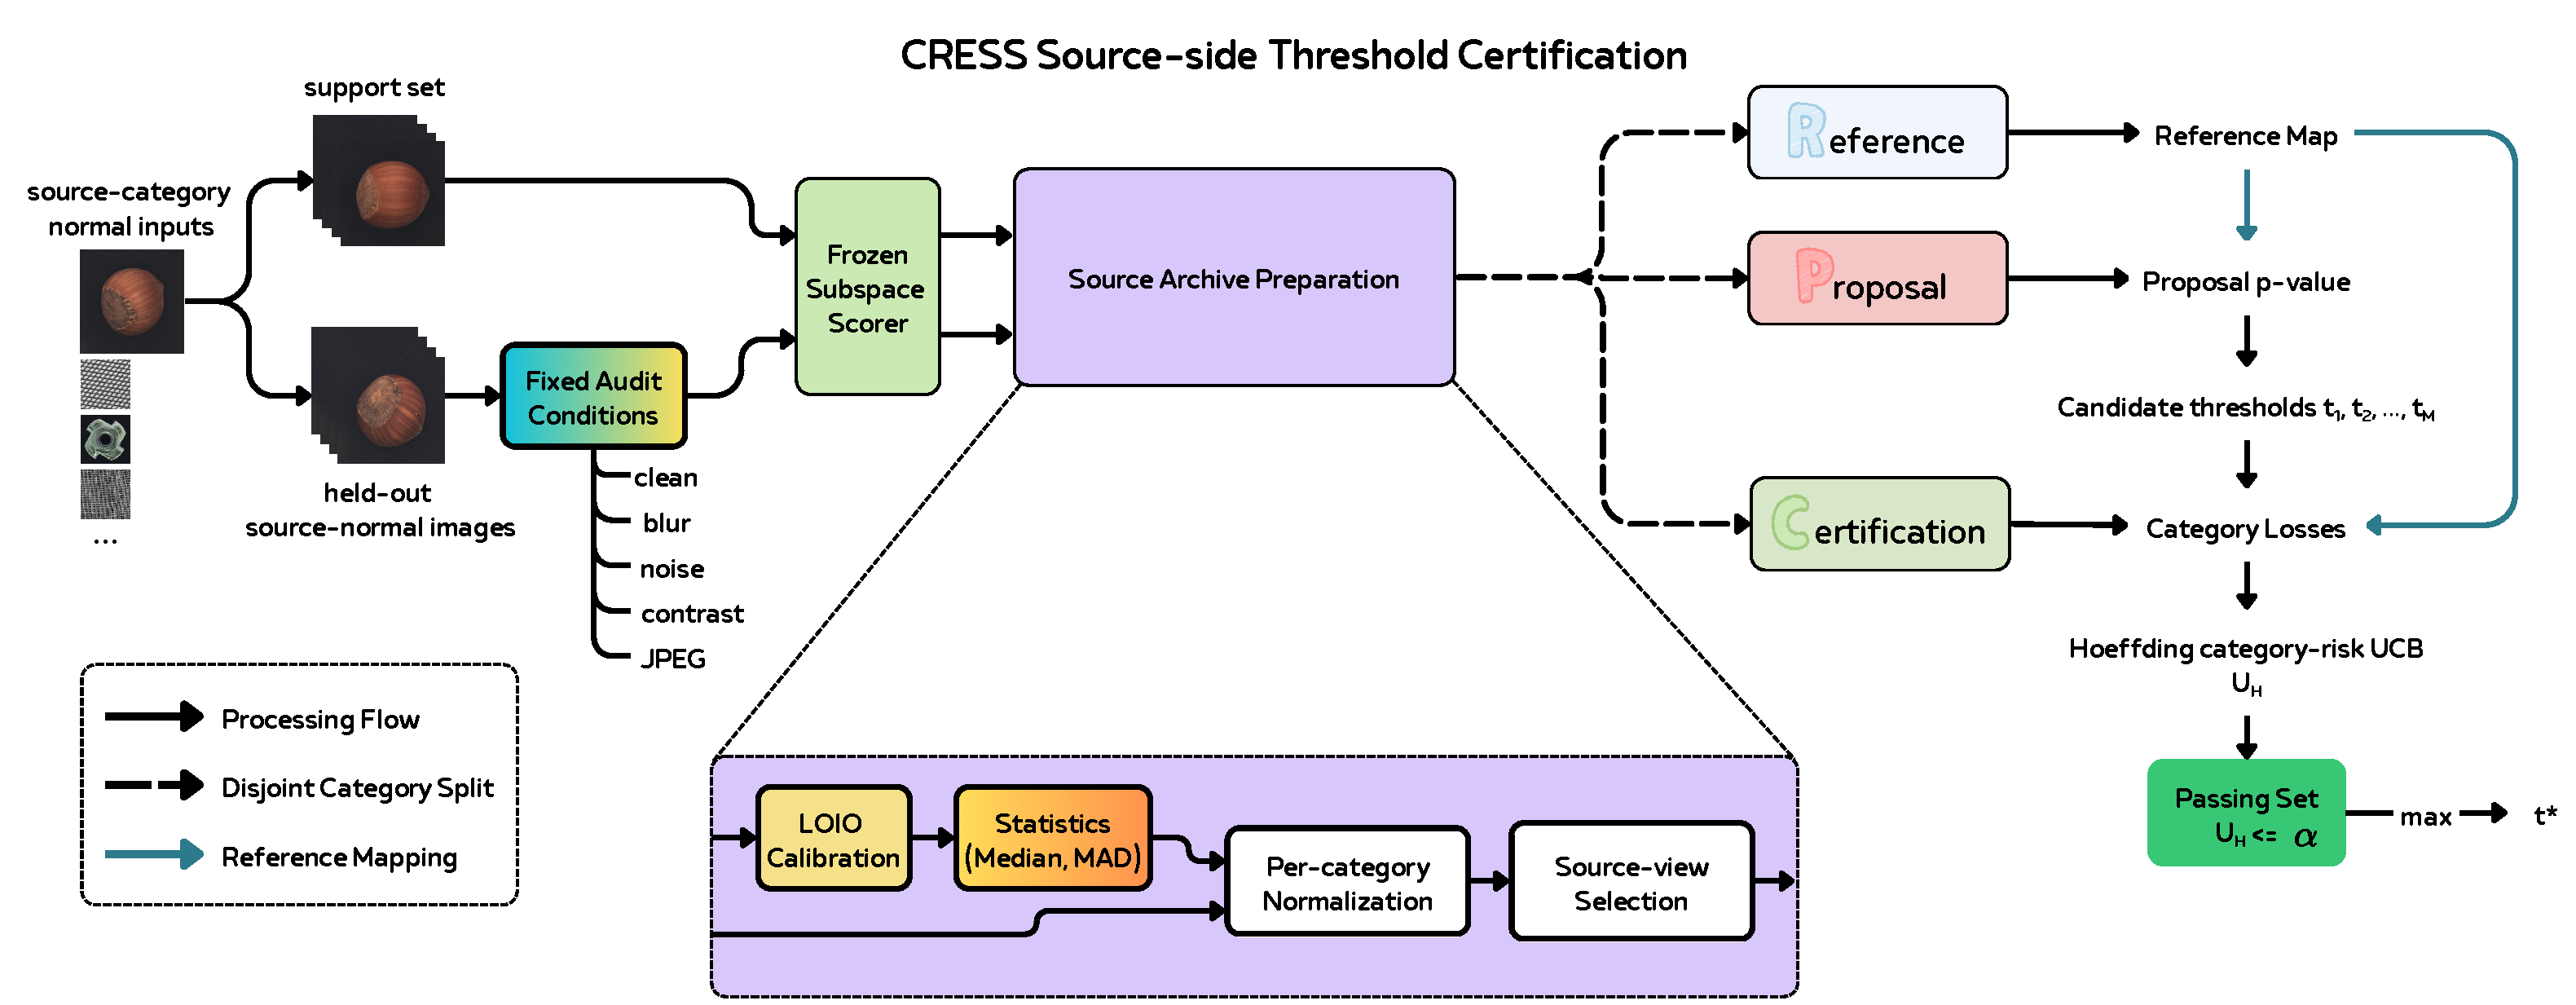
\includegraphics[width=0.98\textwidth]{fig_cress_pipeline}
\caption{CRESS source-side threshold certification. Each non-target source category supplies normal support images for scorer fitting and support-only normalization statistics, together with held-out known-normal views under the predeclared audit conditions. Source-archive preparation normalizes scores before source-view selection; at $k=1$, the declared patch-split support residual replaces LOIO calibration. Eligible source categories are then partitioned disjointly into reference ($\mathcal R$), proposal ($\mathcal P$), and certification ($\mathcal C$) roles. The reference set defines the source-reference map $p_{\mathcal R}$, which is applied to proposal and certification views; the proposal set fixes the candidate family, and the certification set produces category losses for the family-adjusted risk UCB\@. CRESS returns the largest passing threshold or the fail-closed value zero. This is a source-domain certificate; target-category control additionally requires the transfer condition in Corollary~1.}
\label{fig:cress-pipeline}
\end{figure*}

\subsection{Certificate Scope, Feasibility, and Transfer Boundary}
\noindent\textbf{Proposition 1 (conditional source certificate).} For one fixed target, support size and seed, source-view mode, and condition, condition on the reference and proposal stages; under the image model, additionally condition on the fitted certification scorers. Suppose certification units are independent draws from the declared source-unit population: pooled Bernoulli alarm indicators under the image model, or category units that include their support construction and held-out views and yield bounded losses in $[0,1]$ under the category model. Then, with probability at least $1-\delta$, simultaneously across the $A$ levels and both unit definitions, the corresponding source risk of every selected threshold is at most its $\alpha$.

\noindent\emph{Proof.} For a fixed level, unit, and candidate, the one-sided Clopper--Pearson construction or Hoeffding's inequality fails with probability at most $\delta/(2AM)$. A union bound over $M$ candidates, $A$ levels, and two units gives total failure probability at most $\delta$; independence between these bounds is unnecessary. Selection occurs only on this simultaneous event, and the zero fallback has zero alarm risk. \hfill$\square$

\noindent\textbf{Proposition 2 (Hoeffding feasibility).} Under the category-level Hoeffding rule, a positive candidate can pass at level $\alpha$ only if
\begin{equation}\label{eq:cress-feasibility}
    n\geq\frac{\log(2AM/\delta)}{2\alpha^2}.
\end{equation}
\noindent\emph{Proof.} Because $\overline{L}_{\mathcal C}(\tau)\geq0$, the unclipped upper bound is at least $\sqrt{\log(2AM/\delta)/(2n)}$. Requiring it not to exceed $\alpha$ and rearranging proves the claim. \hfill$\square$

\noindent\textbf{Proposition 3 (distribution-free all-zero lower bound).}
Let $\beta\in(0,1)$ and let $L_1,\ldots,L_n$ be iid losses from an arbitrary distribution $P$ on $[0,1]$, with mean $\mu_P$. Let $U_n:[0,1]^n\to[0,1]$ be any deterministic UCB satisfying
\[
    \inf_{P}\Pr_{P^n}\!\left\{\mu_P\leq U_n(L_1,\ldots,L_n)\right\}\geq1-\beta.
\]
Then
\begin{equation}\label{eq:distribution-free-feasibility}
    U_n(0,\ldots,0)\geq1-\beta^{1/n}.
\end{equation}
Consequently, even after observing zero loss in every certification category, $U_n\leq\alpha$ is possible only if
\[
    n\geq\frac{\log\beta}{\log(1-\alpha)}.
\]

\noindent\emph{Proof.}
Write $u=U_n(0,\ldots,0)$ and suppose, for contradiction, that $u<1-\beta^{1/n}$. Choose a Bernoulli distribution with mean $q$ such that $u<q<1-\beta^{1/n}$. Its all-zero sample has probability $(1-q)^n>\beta$. On that event $U_n=u<q=\mu_P$, so the bound fails with probability greater than $\beta$, contradicting uniform $(1-\beta)$ coverage. Rearranging $1-\beta^{1/n}\leq\alpha$ gives the sample-size condition. \hfill$\square$

Proposition~3 shows that the frozen failure is not solely an artifact of Hoeffding looseness. Its Bernoulli counterexample is elementary; the contribution here is to use that necessary condition as an explicit category-budget calculation for transferable anomaly thresholds. Even for one fixed candidate, one level, no image-unit co-reporting, and no multiplicity penalty ($\beta=\delta=0.05$), any deterministic uniformly valid distribution-free bound based only on iid category losses needs at least 14, 29, and 59 categories at $\alpha=0.20$, $0.10$, and $0.05$. These are necessary lower limits, not claims that the corresponding sample sizes suffice for CRESS\@. Under the frozen allocation $\beta=\delta/(2AM)$ with $A=3$ and the most favorable $M=1$, the corresponding lower limits are 22, 46, and 94; the declared Hoeffding rule requires 60, 240, and 958.

An equivalent design interpretation follows by solving Eq.~\eqref{eq:distribution-free-feasibility} for the confidence level. With $n$ all-zero categories, no bound in the scope of Proposition~3 can certify risk at most $\alpha$ with confidence greater than $1-(1-\alpha)^n$. At $\alpha=0.20$, three and four categories therefore support at most 48.8\% and 59.0\% confidence, respectively, in the optimistic multiplicity-free case. Conversely, at 95\% confidence their all-zero UCB floors are 0.632 and 0.527. This restatement quantifies the confidence attainable with the available category budget without treating that budget as sufficient for CRESS\@.

% BEGIN INLINED FILE: tables/tab_certificate_feasibility.tex
\begin{table}[t]
\centering
\caption{Minimum iid certification-category counts required by the all-zero calculations at $\delta=0.05$. The distribution-free rows report the necessary lower bound for deterministic uniformly valid procedures in Proposition~3, first without multiplicity ($\beta=\delta$), then with $\beta=\delta/(2AM)$, $A=3$, and realized family size $M$. ``Hoeffding'' gives Proposition~2. All rows assume zero observed loss; meeting a listed count does not itself guarantee a positive CRESS threshold.}
\label{tab:certificate-feasibility}
\footnotesize
\setlength{\tabcolsep}{4pt}
\begin{tabular}{lrrr}
\toprule
rule / candidates & $\alpha=.20$ & $\alpha=.10$ & $\alpha=.05$ \\
\midrule
Distribution-free, no multiplicity & 14 & 29 & 59 \\
\midrule
Distribution-free, $M=1$  & 22 & 46 & 94 \\
Distribution-free, $M=5$  & 29 & 61 & 125 \\
Distribution-free, $M=20$ & 35 & 74 & 152 \\
\midrule
Hoeffding, $M=1$  & 60 & 240 & 958 \\
Hoeffding, $M=5$  & 80 & 320 & 1,280 \\
Hoeffding, $M=20$ & 98 & 390 & 1,557 \\
\bottomrule
\end{tabular}
\end{table}
% END INLINED FILE: tables/tab_certificate_feasibility.tex

Table~\ref{tab:certificate-feasibility} is a design calculation rather than an empirical result. Proposition~3 is limited to deterministic, uniformly valid, distribution-free upper bounds based solely on iid bounded category losses. Parametric or hierarchical assumptions, informative side data, and randomized confidence procedures require separate validity arguments. Adding independent source-image draws may refine the selected-mixture image analysis, but additional images or repeated support seeds cannot increase the number of independent certification categories. Nor can a different disjoint allocation rescue the current source pools while keeping $\mathcal R$ and $\mathcal P$ nonempty: pools of 14, 11, and 15 eligible categories permit at most 12, 9, and 13 certification categories, respectively, each below the optimistic multiplicity-free requirement of 14 at $\alpha=0.20$.

\noindent\textbf{Corollary 1 (conditional target transfer).} On the event in Proposition~1, the risk of a particular target category under the support construction being evaluated is at most $\alpha$ if, for every proposed threshold, its normal alarm probability is no larger than the corresponding certified source risk. Alternatively, for the category-unit bound, suppose a target category together with its support construction and normal-view sampling mechanism is a fresh independent draw from the same meta-population as the certification-category units. Then the archive-level alarm loss marginalized over that random category draw is at most $\alpha$. Under representative within-category sampling, the same statement applies to the marginal alarm probability of a fresh normal view.

\noindent\emph{Proof.} The first statement follows by source-risk dominance and Proposition~1. If the complete target unit is an independent draw from the same meta-population, its marginal archive-level risk equals the source meta-population risk bounded in Proposition~1. Representative within-category sampling equates the expectation of that archive average with the corresponding fresh-view alarm probability. Neither argument bounds the category-conditional risk of every realized target. \hfill$\square$

Source-risk dominance and iid category sampling are assumptions, not consequences of normalization, source-view selection, or the rank transformation in Eq.~\eqref{eq:cress-source-pvalue}. Thus $\tau^\star$ carries a source-domain certificate. It becomes a guarantee for a particular target only under dominance; iid category sampling supplies the weaker marginal new-category statement. Direct pooled-source conformal, which uses the complete selected source pool with $\tau=\alpha$ and no disjoint proposal or certification stage, is retained as an uncertified empirical reference.
% END INLINED FILE: sections/method.tex
% BEGIN INLINED FILE: sections/experiments.tex
\section{Experiments}\label{sec:experiments}
\subsection{Datasets and Few-Shot Splits}
We evaluate MVTec AD~\cite{mvtec2019} and VisA~\cite{visa2022}. The strict external-transfer audit additionally incorporates MPDD\@. MVTec AD comprises industrial object and texture categories with pixel-level defect masks. VisA contains a broader range of industrial categories and serves as the primary benchmark for full-scale corruption and calibration shift. MPDD provides six metal-part categories for an external stress test that transfers from MVTec to MPDD. Within-MPDD certification is not pursued because the frozen nested implementation requires at least six eligible source categories, whereas excluding one MPDD target leaves five. For each category and seed, one random permutation of the path-sorted normal training images defines nested support sets, so the $k$-shot set is contained in every larger declared set. The CRESS source archive is separate: it consists of held-out known-normal evaluation images from non-target source categories (the \texttt{test/good} partition for MVTec and the corresponding normal partition for VisA and MPDD). Source normal status is therefore used, but target test labels never enter reference construction, threshold proposal, or certification. Unless otherwise specified, $k\in\{1,2,4,8\}$ is employed for the clean accuracy-storage and strict nested studies, whereas the target-only corruption tables use $k\in\{4,8\}$. The $k=1$ strict cells use the declared patch-split support calibration fallback and are interpreted as stress tests; LOIO calibration itself requires $k\geq2$.

\subsection{Evaluation Protocols}
The target-only corruption audit evaluates all test images from all 15 MVTec and 12 VisA categories at $k\in\{4,8\}$ under five support-sampling seeds, with the $k$ sets nested within each seed, and four corruptions. Support images remain clean; each corruption is applied only to evaluation views. Images are represented on $[0,1]$. Gaussian noise adds independent $\mathcal N(0,0.05^2)$ pixel-channel noise and clips the result; blur uses a box-filter radius of one pixel (the declared three-pixel kernel); brightness/contrast applies $\operatorname{clip}(1.15(x-0.5)+0.55,0,1)$; and JPEG uses a quality-60 encode/decode. Each transformed array is clipped, quantized to 8-bit, and stored as a PNG before feature extraction. The noise generator uses the support seed plus the fixed image index, while the other transformations are deterministic. Its primary rank values follow Eq.~\eqref{eq:loio}: calibration scores use LOIO fits and each test score uses the full-support fit. The fold-matched construction is reported only as a sensitivity analysis. Alarm comparisons use the predeclared tolerance $10^{-6}$ to absorb fp32 representation error at attainable grid points.

The primary empirical groups are the target-only corruption audit and the frozen strict nested CRESS audit; the category-count feasibility curves are analytic design calculations. Supporting groups cover clean ranking and storage, PCA64/PCA128 sensitivity, direct pooled-source conformal, and attainable operating levels. The strict nested protocol uses $k\in\{1,2,4,8\}$, seeds from 0 to 4, $\alpha\in\{0.05,0.10,0.20\}$, and clean, Gaussian-noise, blur, brightness/contrast, and JPEG conditions. Its shared score export retains at most 120 evaluation records per category, seed, and condition through deterministic label-stratified sampling, so dataset labels determine the retained evaluation strata. Target labels are then used only to score evaluation outcomes; they do not enter threshold construction. Downstream source construction discards every anomalous source row, so source anomaly scores enter neither the reference map nor proposal or certification losses. The remaining cells use $\rho=0.01$, PCA64, $\delta=0.05$, and realized $M=|\mathcal T|\leq20$. Raw scores are first normalized using support-only statistics; condition-specific source views are then selected or aggregated as defined in Section~\ref{sec:cress-source-construction}. For every target category and seed, the eligible source categories are deterministically split using the frozen $0.50/0.25/0.25$ reference/proposal/certification allocation. This gives 7/3/4 categories for a 14-category within-MVTec source pool, 5/3/3 for an 11-category within-VisA pool, and 7/4/4 for the 15-category MVTec transfer pool. The same category partition is reused across conditions and $k$. The protocol evaluates MVTec and VisA within-dataset, MVTec-to-VisA, and MVTec-to-MPDD under matched-condition, clean-source, condition-agnostic, and mismatched negative-control source selection.

The frozen operational gate first requires a positive category-level threshold in at least 80\% of target cells. It then checks target FAR, power, no-harm versus LOIO, and power gain below the target-only floor. The 80\% cutoff is a predeclared usability criterion, not a confidence level; because the observed rate is zero, any positive cutoff gives the same verdict. The confidence allocation in Proposition~1 applies within each fixed target, seed, source-view mode, and condition cell; it is not a simultaneous 95\% guarantee over the complete experimental grid. Failed cells are retained.

\subsection{Baselines and Ablations}
We compare the inherited PCA residual scorer with a controlled NN memory bank using the same frozen DINOv2 features and few-shot split. PCA64 and PCA128 retain 64 and 128 principal directions, respectively; PCA64 is the default reliability substrate. For the source-assisted study, direct pooled-source conformal is an uncertified baseline: it uses the complete selected source pool with $\tau=\alpha$, but performs no reference, proposal, or certification split and applies no UCB gate. The controlled memory-bank implementation is not an official reproduction of PatchCore or AnomalyDINO; it isolates scoring and storage trade-offs under a common protocol. AnomalyDINO-S (448)~\cite{damm2025anomalydino} is included through values reported under its published protocol. WinCLIP~\cite{winclip2023} is likewise included only through published values because the audit identifies no author-released implementation associated with the cited paper. SubspaceAD is treated as a prior-art guardrail rather than a controlled baseline: the frozen DINOv2 subspace residual is inherited, and the contribution begins with the reliability analysis downstream of that score.

\subsection{Metrics}
Ranking metrics are distinguished from reliability metrics. Image AUROC and AP are calculated from the raw PCA residual score $s(x)$; pixel maps are not certification targets. Reliability is evaluated operationally by empirical FAR at fixed $\alpha$, detection power, alarm precision, the empirical cumulative distribution function (CDF) of normal rank values, and the fraction of cells receiving a positive certified threshold. Storage is quantified as retained ranker state per category. Corruption views are controlled stress tests and are not treated as independent images or as a proxy for all deployment shifts.

\subsection{Reproducibility and Claim Rules}
We conduct all experiments on a single NVIDIA RTX 5090 graphics processing unit (GPU) using PyTorch 2.12.1. DINOv2 patch features are cached in 32-bit floating-point (fp32) format. Reproducibility records include the declared protocol revision, recorded worktree state, DINOv2 source-tree and weight hashes, environment specifications, dataset counts, per-image predictions, base-image identities, support manifests, corruption parameters, source partitions, candidate-threshold bounds, and Secure Hash Algorithm 256-bit (SHA-256) checksums. Automated integrity checks pass for 1,500 MVTec, 1,200 VisA, and 600 MPDD view cells and reject duplicate cells, missing support statistics, or overlap between support and test sets. Reliability methods cannot claim ranking improvement unless the raw score is altered; image-level and category-level certificates are not interchangeable.

OpenAI Codex assisted code review, test generation, and audit scripting. The authors reviewed all changes, and no AI tool generated or altered empirical data.
% END INLINED FILE: sections/experiments.tex
% BEGIN INLINED FILE: sections/results.tex
\section{Results}\label{sec:results}

\subsection{Shift-Induced False-Alarm Inflation}\label{sec:target-only-operation}
% BEGIN INLINED FILE: tables/tab_attainable_alpha.tex
\begin{table*}[pos=t]
\centering
\caption{Target-only LOIO operating points. The floor is the smallest rank value, $1/(k{+}1)$; ``attainable'' is the largest rank-value grid point not exceeding the nominal $\alpha$, or zero if none exists. Within each corruption, FAR and detection power are pooled over categories and seeds; the table then averages the four corruption-specific rates.}
\label{tab:attainable-alpha}
\footnotesize
\setlength{\tabcolsep}{3pt}
\begin{tabular}{llrrrrr}
\toprule
dataset & $k$ & floor & nominal $\alpha$ & attainable & FAR & power \\
\midrule
\multirow{8}{*}{VisA (full)} & \multirow{4}{*}{4} & \multirow{4}{*}{0.200} & 0.01 & 0.000 & 0.000 & 0.000 \\
 & & & 0.05 & 0.000 & 0.000 & 0.000 \\
 & & & 0.10 & 0.000 & 0.000 & 0.000 \\
 & & & 0.20 & 0.200 & 0.142 & 0.595 \\
\cmidrule(lr){2-7}
 & \multirow{4}{*}{8} & \multirow{4}{*}{0.111} & 0.01 & 0.000 & 0.000 & 0.000 \\
 & & & 0.05 & 0.000 & 0.000 & 0.000 \\
 & & & 0.10 & 0.000 & 0.000 & 0.000 \\
 & & & 0.20 & 0.111 & 0.094 & 0.555 \\
\midrule
\multirow{8}{*}{MVTec (full)} & \multirow{4}{*}{4} & \multirow{4}{*}{0.200} & 0.01 & 0.000 & 0.000 & 0.000 \\
 & & & 0.05 & 0.000 & 0.000 & 0.000 \\
 & & & 0.10 & 0.000 & 0.000 & 0.000 \\
 & & & 0.20 & 0.200 & 0.278 & 0.880 \\
\cmidrule(lr){2-7}
 & \multirow{4}{*}{8} & \multirow{4}{*}{0.111} & 0.01 & 0.000 & 0.000 & 0.000 \\
 & & & 0.05 & 0.000 & 0.000 & 0.000 \\
 & & & 0.10 & 0.000 & 0.000 & 0.000 \\
 & & & 0.20 & 0.111 & 0.200 & 0.868 \\
\bottomrule
\end{tabular}
\end{table*}
% END INLINED FILE: tables/tab_attainable_alpha.tex
% BEGIN INLINED FILE: tables/tab_false_alarm_control.tex
\begin{table*}[pos=t]
\centering
\caption{Target-only LOIO FAR, detection power, and alarm precision at the first reported attainable level, $\alpha{=}0.20$. Results use five support-sampling seeds with support sets nested across $k$, are pooled over images within each dataset, corruption, and $k$, and retain every normal and anomalous test image. Alarms fire when the rank value satisfies $p\le\alpha$, using the comparison tolerance described in the text.}
\label{tab:false-alarm-control}
\footnotesize
\setlength{\tabcolsep}{3pt}
\begin{tabular}{llrrrr}
\toprule
dataset & corruption & $k$ & FAR & power & precision \\
\midrule
\multirow{8}{*}{VisA (full)} & \multirow{2}{*}{blur} & 4 & 0.144 & 0.606 & 0.825 \\
 & & 8 & 0.094 & 0.566 & 0.870 \\
\cmidrule(lr){2-6}
 & \multirow{2}{*}{bright/contr.} & 4 & 0.146 & 0.596 & 0.821 \\
 & & 8 & 0.098 & 0.557 & 0.864 \\
\cmidrule(lr){2-6}
 & \multirow{2}{*}{Gaussian noise} & 4 & 0.133 & 0.575 & 0.829 \\
 & & 8 & 0.081 & 0.538 & 0.881 \\
\cmidrule(lr){2-6}
 & \multirow{2}{*}{JPEG} & 4 & 0.145 & 0.602 & 0.822 \\
 & & 8 & 0.104 & 0.559 & 0.858 \\
\midrule
\multirow{8}{*}{MVTec (full)} & \multirow{2}{*}{blur} & 4 & 0.219 & 0.880 & 0.904 \\
 & & 8 & 0.139 & 0.870 & 0.936 \\
\cmidrule(lr){2-6}
 & \multirow{2}{*}{bright/contr.} & 4 & 0.214 & 0.882 & 0.906 \\
 & & 8 & 0.133 & 0.870 & 0.939 \\
\cmidrule(lr){2-6}
 & \multirow{2}{*}{Gaussian noise} & 4 & 0.341 & 0.873 & 0.857 \\
 & & 8 & 0.281 & 0.860 & 0.878 \\
\cmidrule(lr){2-6}
 & \multirow{2}{*}{JPEG} & 4 & 0.336 & 0.883 & 0.860 \\
 & & 8 & 0.248 & 0.872 & 0.892 \\
\bottomrule
\end{tabular}
\end{table*}
% END INLINED FILE: tables/tab_false_alarm_control.tex

Table~\ref{tab:attainable-alpha} first separates unattainable nominal levels from observed false-alarm behavior. With $k=4$, the smallest rank value is $1/(k+1)=0.2$, so nominal levels 0.01, 0.05, and 0.10 cannot raise an alarm. With $k=8$, the floor decreases to $1/9\approx0.111$, but the same three levels remain below it. Their zero FAR and power values are finite-resolution artifacts, not evidence of conservative false-alarm control.

At nominal $\alpha=0.20$, the effective threshold is 0.20 for $k=4$ but only $1/9$ for $k=8$, because $1/9$ is the largest $k=8$ grid point not exceeding 0.20. On VisA, the aggregate FAR/power pairs are 0.142/0.595 at $k=4$ and 0.094/0.555 at $k=8$; on MVTec they are 0.278/0.880 and 0.200/0.868. These aggregates first pool images over categories and five support-sampling seeds within each corruption and then average the four corruption-specific rates. Thus the MVTec $k=8$ average equals the requested 0.20 budget but exceeds the 0.111 tie-free discrete reference at its effective threshold; it is not an aggregate violation of the requested budget, although the expected finite-grid conservatism is absent. The nominal level induces different effective thresholds across $k$, while the empirical FAR itself is not restricted to the rank-value grid.

Table~\ref{tab:false-alarm-control} resolves the aggregate by corruption. The headline 0.341 is the empirical FAR on Gaussian-corrupted MVTec at $k=4$. It is neither the MVTec average nor a population false-alarm probability. It is the largest dataset-level aggregate in the frozen grid and is approximately 1.7 times the nominal 0.20. Category-level FARs are heterogeneous: after pooling within category over the five seeds, the median is 0.215, the interquartile range is 0.169 to 0.481, and 9 of 15 categories exceed 0.20. Thus, the aggregate is neither universal across categories nor attributable to only one category. JPEG compression is similarly anti-conservative at 0.336. At $k=8$, blur and brightness/contrast are conservative at 0.139 and 0.133, whereas Gaussian noise and JPEG compression remain above nominal at 0.281 and 0.248. Increasing $k$ mitigates but does not eliminate the mismatch.

VisA behaves differently: FAR remains between 0.133 and 0.146 at $k=4$ and between 0.081 and 0.104 at $k=8$. The shift effect is therefore dataset- and condition-dependent, not a universal inflation result. Power remains nonzero at every displayed operating point; precision is descriptive because it depends on benchmark anomaly prevalence. Because fp32 and double-precision representations of 0.2 differ slightly, an exact mixed-precision comparison can inadvertently exclude floor-level alarms. All reported thresholding uses the fixed numerical tolerance declared in the protocol.

The normal-rank audit explains the direction of these deviations. Under the relevant exchangeability conditions, a valid conformal p-value satisfies $P(p\leq\alpha)\leq\alpha$ for normal data. Equation~\eqref{eq:loio} does not assume those conditions, so we compare its conformal-form rank values with that reference rather than presuming validity. Because a $k$-score rank value lies on the grid $\{j/(k+1)\}$, a continuous Kolmogorov--Smirnov test against $U(0,1)$ is inappropriate. Figure~\ref{fig:uniformity} instead compares the empirical normal-rank CDF with the tie-free discrete-uniform benchmark at each attainable point. Under valid exchangeability, ties can make the rank values more conservative, so the population CDF need only lie at or below this benchmark; the finite pooled CDF remains descriptive. VisA at $k=4$ is conservative, with the largest displayed negative gap, $-0.087$, occurring under blur at 0.6; at $k=8$, its first grid point remains conservative although small anti-conservative gaps appear at higher grid points. MVTec is anti-conservative at both $k$ values, especially under Gaussian noise and JPEG compression. For Gaussian-corrupted MVTec at $k=4$, $\widehat F(0.2)=0.341$ versus the benchmark value 0.20, and the gap grows to 0.204 at the 0.4 grid point.

Rows share calibration sets, categories, and repeated test images across seeds. We therefore treat the CDF comparison as descriptive and do not attach an iid goodness-of-fit test to the pooled points. The results show that corrupted normal scores increase relative to clean support calibration scores, but do not identify a causal mechanism. On full MVTec at $k=4$, the fold-matched LOIO sensitivity increases clean FAR from 0.212 to 0.257 and power from 0.880 to 0.906. This direction is consistent with the full-support test fit suppressing alarms relative to the $k-1$ calibration fits: the retained asymmetry can make the original audit appear more conservative, but does not establish validity. Fold matching likewise fails to restore false-alarm control.

\begin{figure*}[pos=t]
    \centering
    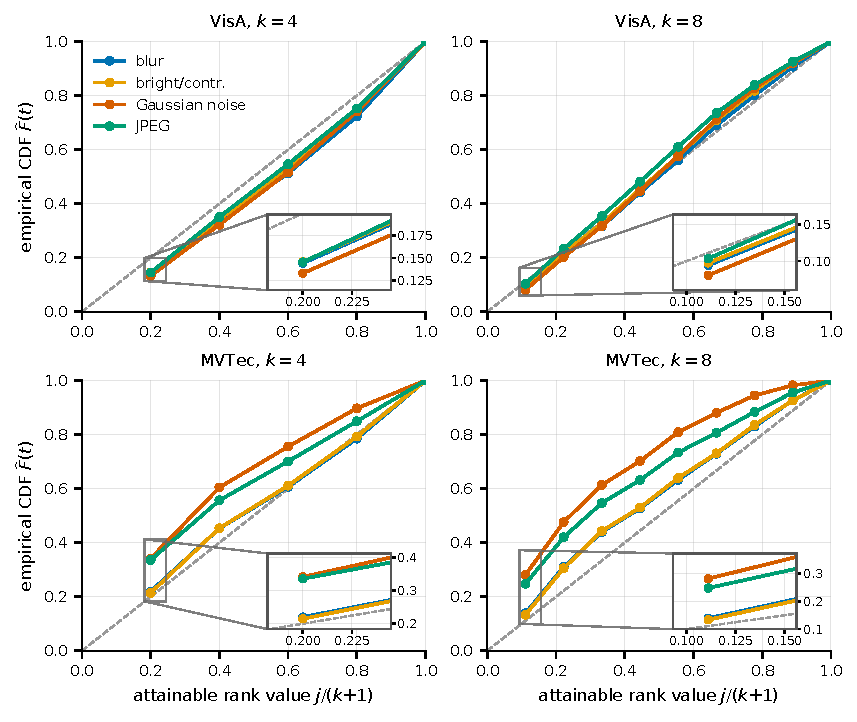
\includegraphics[width=0.92\linewidth]{fig_uniformity_cdf}
    \caption{Empirical CDF of normal-image LOIO rank values at each attainable point $j/(k{+}1)$ versus the tie-free discrete-uniform benchmark (dashed diagonal), using five support-sampling seeds. Valid ties may move the population CDF below this benchmark. Points above the diagonal indicate excess empirical false alarms relative to the benchmark; lower-right insets and connector rays enlarge the first attainable grid region.}
    \label{fig:uniformity}
\end{figure*}

\subsection{Category-Count Feasibility}\label{sec:category-feasibility-results}
Figure~\ref{fig:certificate-feasibility} and Table~\ref{tab:certificate-feasibility} are analytic design calculations, not fitted learning curves. In the optimistic multiplicity-free case, the all-zero distribution-free floor crosses $\alpha=0.20$, 0.10, and 0.05 only at 14, 29, and 59 iid category draws. These counts are necessary within the scope of Proposition~3; they are not sufficient sample sizes for a positive CRESS threshold. The frozen family allocation with $A=3$ and favorable $M=1$ increases the lower limits to 22, 46, and 94, while the corresponding Hoeffding rule requires 60, 240, and 958.

Candidate multiplicity widens the gap. At the cap $M=20$, the family-adjusted distribution-free lower limits become 35, 74, and 152, and the Hoeffding requirements become 98, 390, and 1,557. The three or four certification categories available in the frozen audit lie below even the most optimistic 14-category requirement at $\alpha=0.20$. This is not merely an artifact of assigning 25\% of the source pool to certification: any disjoint split with nonempty reference and proposal roles can allocate at most 12 MVTec, 9 VisA, or 13 transfer-source categories to certification, still below 14. This comparison answers a feasibility question before any target performance is inspected: within the deterministic distribution-free class of Proposition~3, a nonzero certificate of marginal new-category risk is unavailable from the present source pools, even under zero observed category loss. The result does not rule out parametric, hierarchical, randomized, or side-information procedures; such methods require separate assumptions and validity arguments.

The confidence-level view makes the shortage concrete. At $\alpha=0.20$, three all-zero categories can support at most 48.8\% confidence and four can support at most 59.0\% confidence under the optimistic multiplicity-free assumptions of Proposition~3. If 95\% confidence is fixed instead, the corresponding all-zero UCB floors are 0.632 and 0.527. Both are already far above 0.20 before candidate multiplicity or image-unit co-reporting is charged.

\subsection{CRESS Boundary Test: Categories versus Images}\label{sec:cress-strict-results}
% BEGIN INLINED FILE: tables/tab_strict_nested_sc3r.tex
\begin{table*}[t]
\centering
\caption{Frozen strict CRESS audit over 960 job $\times$ source-view $\times$ $k$ $\times$ $\alpha$ $\times$ condition configurations, 240 per source-to-target job. Each configuration contains 75 MVTec, 60 VisA, or 30 MPDD target-category/seed cells; hence ``nonzero frac.'' pools 18,000, 14,400, or 7,200 cells per indicated job. ``Min UCB'' is the smallest observed candidate bound. Category and image rows target different estimands; image rows assume the idealized iid source-image model.}
\label{tab:strict-cress}
\footnotesize
\setlength{\tabcolsep}{5pt}
\begin{tabular}{llrrrl}
\toprule
source $\rightarrow$ target & certification unit & units/cell & min UCB & nonzero frac. & interpretation \\
\midrule
MVTec $\rightarrow$ MVTec & category & 4 & 0.950 & 0.000 & category-unit gate fails \\
VisA $\rightarrow$ VisA & category & 3 & 1.000 & 0.000 & category-unit gate fails \\
MVTec $\rightarrow$ VisA & category & 4 & 0.961 & 0.000 & category-unit gate fails \\
MVTec $\rightarrow$ MPDD & category & 4 & 0.986 & 0.000 & category-unit gate fails \\
\midrule
MVTec $\rightarrow$ MVTec & source image & 75 to 191 & 0.039 & 0.367 & iid-image sensitivity \\
VisA $\rightarrow$ VisA & source image & 150 to 180 & 0.042 & 0.603 & iid-image sensitivity \\
MVTec $\rightarrow$ VisA & source image & 72 to 159 & 0.048 & 0.415 & iid-image sensitivity \\
MVTec $\rightarrow$ MPDD & source image & 81 to 190 & 0.040 & 0.370 & iid-image sensitivity \\
\bottomrule
\end{tabular}
\end{table*}
% END INLINED FILE: tables/tab_strict_nested_sc3r.tex
% BEGIN INLINED FILE: tables/tab_pooled_source_conformal.tex
\begin{table}[pos=t]
\centering
\caption{Direct pooled-source conformal under matched-condition selection. Entries are unweighted means of within-target-cell rates over categories, $k\in\{1,2,4,8\}$, five support seeds, and five conditions. The complete selected source pool uses $\tau=\alpha$ without a reference/proposal/certification split; this is an empirical, uncertified baseline.}
\label{tab:pooled-source-conformal}
\footnotesize
\setlength{\tabcolsep}{4pt}
\begin{tabular}{lrrr}
\toprule
source $\rightarrow$ target & $\alpha$ & FAR & power \\
\midrule
\multirow{3}{*}{MVTec $\rightarrow$ MVTec}
 & 0.05 & 0.075 & 0.404 \\
 & 0.10 & 0.131 & 0.566 \\
 & 0.20 & 0.242 & 0.754 \\
\cmidrule(lr){1-4}
\multirow{3}{*}{VisA $\rightarrow$ VisA}
 & 0.05 & 0.060 & 0.320 \\
 & 0.10 & 0.111 & 0.466 \\
 & 0.20 & 0.208 & 0.639 \\
\cmidrule(lr){1-4}
\multirow{3}{*}{MVTec $\rightarrow$ VisA}
 & 0.05 & 0.028 & 0.171 \\
 & 0.10 & 0.048 & 0.282 \\
 & 0.20 & 0.099 & 0.441 \\
\cmidrule(lr){1-4}
\multirow{3}{*}{MVTec $\rightarrow$ MPDD}
 & 0.05 & 0.030 & 0.186 \\
 & 0.10 & 0.066 & 0.283 \\
 & 0.20 & 0.157 & 0.423 \\
\bottomrule
\end{tabular}
\end{table}
% END INLINED FILE: tables/tab_pooled_source_conformal.tex

Table~\ref{tab:strict-cress} tests whether the analytic shortage binds in the frozen CRESS protocol. The 960 gate configurations comprise four source-to-target jobs, four source-view modes, four $k$ values, three $\alpha$ levels, and five conditions, or 240 per job; each aggregates target categories and five support seeds. They are repeated configurations in a frozen grid, not independent statistical trials, and Proposition~1 supplies a per-cell rather than grid-wide simultaneous guarantee. Category-unit certification assigns $\tau^\star=0$ to every underlying cell, and no configuration reaches the required 80\% nonzero-threshold rate. The smallest candidate UCB is 0.950 on MVTec, 1.000 on VisA, 0.961 for MVTec-to-VisA, and 0.986 for transfer from MVTec to MPDD\@. Even the smallest value is 4.75 times the largest tested $\alpha=0.20$.

The fail-closed result agrees with the design calculation and is not a compute or optimization failure. Proposition~2 requires at least 60 categories for the favorable $M=1$ Hoeffding gate at $\alpha=0.20$, while Proposition~3 requires at least 14 categories even for the optimistic multiplicity-free distribution-free case and at least 22 under the favorable frozen allocation. Only three or four certification categories are available. Because the operational gate is conjunctive, the zero nonzero-threshold rate already determines failure; downstream target-performance checks cannot convert $\tau^\star=0$ into a usable alarm threshold. The same zero-threshold conclusion holds when the $k=1$ stress cells are excluded and only $k\in\{2,4,8\}$ is retained, so it does not depend on the patch-split fallback. The strict experiment therefore shows a fail-closed outcome consistent with the predicted category-count boundary throughout the declared grid; it does not provide 960 replications of the theoretical result.

The image-unit block changes both the sample size and the estimand. Under its idealized conditional iid source-image assumption, 72 to 191 selected source-image units per cell reduce the smallest UCB to 0.039 to 0.048. Positive thresholds occur in 36.7\% of MVTec, 60.3\% of VisA, 41.5\% of MVTec-to-VisA, and 37.0\% of MVTec-to-MPDD target cells. These rates remain below the 80\% operational gate overall. More importantly, their risk refers to image draws from the selected source mixture. The additional images do not create independent categories and cannot be relabeled as evidence for a marginal new-category certificate. Thus, the same source data can be informative for the image-mixture estimand and insufficient for a distribution-free category-transfer estimand.

Table~\ref{tab:pooled-source-conformal} reports direct pooled-source conformal as an uncertified empirical reference. It uses the complete selected source pool with $\tau=\alpha$ and no disjoint reference, proposal, or certification categories. Entries are unweighted means of within-target-cell rates, so categories and support seeds receive equal weight regardless of image count. Under matched-condition selection, mean FAR exceeds nominal within MVTec and VisA at every displayed level; transfer is more conservative and less powerful. Direct pooling supplies finer operating points than target-only LOIO, but characterizes empirical risk under the selected source mixture rather than certified new-category risk.

\subsection{Supporting Ranking Substrate and Storage}
% BEGIN INLINED FILE: tables/tab_clean_efficiency.tex
\begin{table*}[pos=t]
\centering
\caption{Clean image-level ranking performance and category-specific ranker state in mebibytes (MiB). Controlled DINOv2 NN and PCA64/PCA128 share our feature, split, metric, and storage-accounting protocol and are averaged over categories and five seeds. AnomalyDINO-S (448) and WinCLIP values are reported in~\cite{damm2025anomalydino,winclip2023} under their respective protocols. Bold marks the best value only among common-protocol rows in each dataset/$k$ block. ``--'' denotes not evaluated, N/C not directly comparable, and N/R not reported.}
\label{tab:clean-efficiency}
\setlength{\tabcolsep}{2.4pt}
\footnotesize
\begin{tabular}{lllrrr}
\toprule
Dataset & $k$ & Method & AUROC $\uparrow$ & AP $\uparrow$ & MiB $\downarrow$ \\
\midrule
\multirow{11}{*}{MVTec}
& \multirow{4}{*}{1} & AnomalyDINO-S (reported) & 0.965 & 0.981 & -- \\
& & WinCLIP (reported) & 0.931 & N/C & N/R \\
& & Controlled DINOv2 NN & \textbf{0.914} & \textbf{0.952} & 2.005 \\
& & PCA64 (controlled) & 0.904 & 0.951 & \textbf{0.095} \\
\cmidrule(lr){2-6}
& \multirow{4}{*}{4} & AnomalyDINO-S (reported) & 0.976 & 0.984 & -- \\
& & WinCLIP (reported) & 0.952 & N/C & N/R \\
& & Controlled DINOv2 NN & \textbf{0.942} & \textbf{0.967} & 6.000 \\
& & PCA64 (controlled) & 0.937 & \textbf{0.967} & \textbf{0.095} \\
\cmidrule(lr){2-6}
& \multirow{3}{*}{8} & AnomalyDINO-S (reported) & 0.980 & 0.990 & -- \\
& & Controlled DINOv2 NN & \textbf{0.948} & 0.970 & 6.000 \\
& & PCA64 (controlled) & 0.945 & \textbf{0.972} & \textbf{0.095} \\
\midrule
\multirow{14}{*}{VisA}
& \multirow{5}{*}{1} & AnomalyDINO-S (reported) & 0.856 & 0.866 & -- \\
& & WinCLIP (reported) & 0.838 & N/C & N/R \\
& & Controlled DINOv2 NN & 0.804 & 0.809 & 2.005 \\
& & PCA64 (controlled) & 0.823 & 0.834 & \textbf{0.095} \\
& & PCA128 (controlled) & \textbf{0.834} & \textbf{0.842} & 0.189 \\
\cmidrule(lr){2-6}
& \multirow{5}{*}{4} & AnomalyDINO-S (reported) & 0.913 & 0.918 & -- \\
& & WinCLIP (reported) & 0.873 & N/C & N/R \\
& & Controlled DINOv2 NN & 0.862 & 0.861 & 6.000 \\
& & PCA64 (controlled) & 0.870 & 0.883 & \textbf{0.095} \\
& & PCA128 (controlled) & \textbf{0.885} & \textbf{0.895} & 0.189 \\
\cmidrule(lr){2-6}
& \multirow{4}{*}{8} & AnomalyDINO-S (reported) & 0.926 & 0.929 & -- \\
& & Controlled DINOv2 NN & 0.873 & 0.870 & 6.000 \\
& & PCA64 (controlled) & 0.882 & 0.894 & \textbf{0.095} \\
& & PCA128 (controlled) & \textbf{0.897} & \textbf{0.905} & 0.189 \\
\bottomrule
\end{tabular}
\end{table*}
% END INLINED FILE: tables/tab_clean_efficiency.tex

Table~\ref{tab:clean-efficiency} verifies that the reliability conclusions are studied on a viable, compact ranking substrate. The reported AnomalyDINO-S (448) results use that method's published protocol and therefore serve as external accuracy references rather than evidence of superiority under our controlled protocol. WinCLIP is likewise a cited reference: its paper reports AUROC and area under the precision-recall curve (AUPR) at one and four shots, but not an AP implementation verified to match ours. We mark its AP entries N/C instead of mixing the reported AUPR values into the controlled AP comparison. WinCLIP also does not report category-specific storage under our accounting or an eight-shot result.

Relative to the controlled DINOv2 NN ranker, PCA64 AUROC is lower by 0.011, 0.005, and 0.003 on MVTec and higher by 0.019, 0.008, and 0.009 on VisA at $k=1,4,8$, respectively. It is a compact supporting ranker, not a ranking contribution or state-of-the-art claim. Evaluated only on VisA, PCA128 improves mean AUROC over PCA64 by 0.011, 0.016, and 0.014. Differences use unrounded values. Boldface compares common-protocol rows only; external references are excluded.

\emph{Storage accounting.} Storage excludes the shared frozen DINOv2 ViT-S/14 backbone. With $d=384$ fp32 features, the PCA mean and basis require $(m+1)d$ scalars: 0.095\,MiB for PCA64 and 0.189\,MiB for PCA128. Historical PCA128 artifacts include a 0.566\,MiB calibration wrapper, but raw ranking uses only PCA residuals; Table~\ref{tab:clean-efficiency} therefore counts the 0.189\,MiB ranker state. Support-normalization scalars are negligible at the displayed precision. The controlled memory bank stores 2.005\,MiB at $k=1$ and caps at 4096 vectors, or 6.000\,MiB, thereafter. CRESS retains normalized scalar reference scores and partition metadata rather than source patch features. We make no runtime claim.

The clean benchmark uses max pooling, whereas the conformal pipeline uses the top-$1\%$ mean as a smoother operational score. Table~\ref{tab:agg-ablation} in Appendix~\ref{app:tables} probes this choice on three MVTec and four VisA categories over three seeds. Across the displayed rows, the largest AUROC difference between either paper choice and the best tested aggregator is 0.018; moderate top-fraction pooling outperforms max on MVTec, whereas top-$0.5\%$ is best on VisA. This limited subset supports the use of a smoothed operational score but does not establish full-dataset invariance to aggregation. Table~\ref{tab:clean-efficiency} is therefore evidence that the inherited substrate is compact and viable under its declared clean protocol; it is not used to attribute any reliability difference to the PCA ranker.
% END INLINED FILE: sections/results.tex
% BEGIN INLINED FILE: sections/limitations.tex
\section{Limitations}\label{sec:limitations}
The feasibility result has a deliberately narrow statistical scope. Proposition~3 applies to deterministic, uniformly valid, distribution-free UCBs based only on iid bounded category losses. It does not rule out nonvacuous certification from fewer categories under pre-specified parametric or hierarchical models, informative side data, or randomized procedures. Such approaches exchange distribution-free generality for additional assumptions and require their own coverage analyses. The counts 14, 29, and 59 are optimistic necessary limits without multiplicity, not sufficient sample sizes for CRESS\@. The frozen family allocation and declared Hoeffding rule require more. Proposition~1 controls its declared candidate family within one fixed target/seed/source-view/condition cell; the study does not claim one simultaneous 95\% event over all reported cells.

The category interpretation also depends on the unit definition. The strict audit contains only three or four certification categories, and repeated images, corruption views, or support seeds do not constitute additional independent category draws. Image-unit bounds under the selected-mixture iid model therefore address a different estimand rather than a partial certificate for a new category. The benchmark archive is stratified by category, and alarms within a category share a support-fitted scorer; consequently, iid pooled alarm indicators are an idealized sensitivity assumption, not a design-based property of the archive. CRESS certifies source-domain risk under the assumptions of Proposition~1. The benchmark categories are a fixed heterogeneous collection, so their interpretation as iid draws from a source-category meta-population is a modeling assumption rather than an empirically testable fact in these data. A category unit includes its support construction as well as its held-out views. Moreover, the observed $L_c$ values are finite archive averages; interpreting their meta-population mean as the alarm probability of a fresh normal view requires the within-category archive to represent the declared deployment distribution. Applying the selected threshold to a particular target additionally requires source-risk dominance. An independent target draw from the same category meta-population supports only risk marginalized over that draw; it does not control every realized category. Support-only normalization and source-view selection establish neither condition. Matched source selection also assumes reliable condition metadata.

The empirical evidence is limited to MVTec, VisA, and MPDD\@. The controlled shift study covers Gaussian noise, blur, brightness/contrast, and JPEG compression, not the full range of temporal drift, sensor replacement, process changes, correlated failures, or deployment prevalence. The empirical FAR of 0.341 is the largest dataset-level aggregate in this frozen synthetic-corruption grid, not a population failure probability or a universal response to Gaussian noise. CRESS also assumes access to a separately declared archive of known-normal, held-out views from non-target source categories; in these benchmarks those views come from the normal evaluation partition. This source-assisted setup is therefore not the conventional target-category training-only benchmark protocol, although target test labels and images remain excluded from threshold construction. The image-unit sensitivity additionally assumes independent source-image draws; repeated or correlated production images would reduce its effective evidence. Prospective factory evidence is needed to determine whether the same failure mode and category-count assumptions hold under real operational shifts.

Finally, the frozen DINOv2 PCA residual is an inherited ranking substrate. Reported AnomalyDINO-S and WinCLIP results follow different protocols and serve as external references; the paper does not claim ranking state of the art. LOIO calibration and full-support test residuals remain asymmetric, and the pooled discrete-grid audit diagnoses rather than restores exchangeability. We therefore restrict the efficiency comparison to explicitly accounted category-specific storage and make no runtime claim.
% END INLINED FILE: sections/limitations.tex
% BEGIN INLINED FILE: sections/conclusion.tex
\section{Conclusion and Future Work}\label{sec:conclusion}
This study has established that the reliability of few-shot anomaly thresholds depends on both the amount and the statistical unit of normal evidence. At nominal $\alpha=0.20$, target-only LOIO reaches an empirical FAR of 0.341 on Gaussian-corrupted MVTec at $k=4$, showing that an attainable operating point need not remain stable under shift. The finite floor $1/(k+1)$ explains when a target-only rule is structurally silent, but crossing that floor does not supply an exchangeability guarantee.

The category-count analysis has quantified the separate obstacle faced by source-assisted certification. With all category losses zero, optimistic multiplicity-free certification by a deterministic, uniformly valid, distribution-free 95\% UCB requires at least 14, 29, and 59 iid category draws at $\alpha=0.20$, 0.10, and 0.05. These are necessary lower limits, not sufficient budgets for CRESS\@. The frozen allocation and Hoeffding rule require more, whereas the strict audit provides only three or four certification categories. Even a certification-heavy reallocation with nonempty reference and proposal roles provides at most 9 to 13 categories, so changing the split cannot meet the optimistic 14-category limit. Category-unit certification consequently assigns $\tau^\star=0$ to every target cell across all 960 frozen configurations, which share the same boundary and are not independent trials. In contrast, image-unit analyses under the idealized selected-mixture iid model select positive thresholds in 36.7\% to 60.3\% of target cells, but target the selected source mixture rather than marginal risk over a new-category draw.

The practical contribution is therefore a study-design discipline: distinguish ranking from threshold reliability, report attainable rather than nominal operating points, audit normal false alarms under declared shifts, define the certification unit before observing results, and justify iid category sampling when the claim concerns a new category. Future work should collect category-rich source archives or introduce explicit parametric, hierarchical, or side-information assumptions with independently verified validity. It should also test real production shifts, temporal dependence, condition-estimation error, and end-to-end deployment cost. These directions can improve usefulness, but they should not relabel repeated images as category evidence, confuse marginal with category-conditional risk, or convert a source-domain certificate into unconditional target control.
% END INLINED FILE: sections/conclusion.tex
% BEGIN INLINED FILE: sections/appendix.tex
\appendix
\section{Supplementary tables}\label{app:tables}
This appendix reports the subset aggregation-sensitivity ablation summarized in Section~\ref{sec:results}.

% BEGIN INLINED FILE: tables/tab_agg_ablation.tex
\begin{table}[!ht]
\centering
\caption{Aggregation-sensitivity ablation for clean image AUROC under max and top-$\rho$ mean pooling. Results average three MVTec categories (bottle, cable, and hazelnut) or four VisA categories (candle, cashew, pcb1, and pipe fryum) over seeds from 0 to 2. Bold marks the best tested aggregator in each row. This subset analysis diagnoses sensitivity within the displayed grid; it is not a full-dataset ranking comparison.}
\label{tab:agg-ablation}
\footnotesize
\setlength{\tabcolsep}{4pt}
\begin{tabular}{llrrrrr}
\toprule
dataset & $k$ & max & top-0.5\% & top-1\% & top-2\% & top-5\% \\
\midrule
\multirow{2}{*}{MVTec} & 4 & 0.9571 & 0.9638 & 0.9667 & \textbf{0.9693} & 0.9621 \\
 & 8 & 0.9578 & 0.9685 & 0.9740 & \textbf{0.9759} & 0.9727 \\
\midrule
\multirow{2}{*}{VisA} & 4 & 0.9039 & \textbf{0.9101} & 0.9038 & 0.8944 & 0.8806 \\
 & 8 & 0.9101 & \textbf{0.9200} & 0.9147 & 0.9071 & 0.8941 \\
\bottomrule
\end{tabular}
\end{table}
% END INLINED FILE: tables/tab_agg_ablation.tex
\FloatBarrier
% END INLINED FILE: sections/appendix.tex
% BEGIN INLINED FILE: sections/declarations.tex
% Add author-specific \credit{} declarations in main.tex after both authors
% approve the CRediT roles, then restore \section*{CRediT authorship contribution
% statement} and \printcredits here. Attribution is intentionally not inferred.

\section*{Declaration of competing interest}
The authors declare that they have no known competing financial interests or personal relationships that could have appeared to influence the work reported in this paper.

\section*{Data availability}
The datasets analyzed during the current study are publicly available from the \href{https://www.mvtec.com/company/research/datasets/mvtec-ad}{MVTec AD dataset page}, the \href{https://github.com/amazon-science/spot-diff}{VisA repository}, and the \href{https://github.com/stepanje/MPDD}{MPDD repository}. Derived per-image predictions, evaluation summaries, sampling and source-partition manifests, and checksums are available in the \href{https://github.com/OxyzGiaHuy/AD}{project repository}.

\section*{Code availability}
The experimental code, corruption pipeline, integrity audits, and table and figure generators are available in the \href{https://github.com/OxyzGiaHuy/AD}{project repository}. The primary GPU run uses frozen scientific revision \href{https://github.com/OxyzGiaHuy/AD/commit/e7f175990b02aa3cbdb7c92250d57c0272abef9d}{\texttt{e7f175990b02}}; its complete result archive is recorded at revision \href{https://github.com/OxyzGiaHuy/AD/commit/74fdfd00f3480f3bc5db42e29bc51ec0768ab881}{\texttt{74fdfd00f348}}.

\section*{Declaration of generative AI and AI-assisted technologies in the manuscript preparation process}
During the preparation of this work, the authors used OpenAI Codex to support code review, software-test generation, reproducibility checks, statistical claim auditing, manuscript structuring and drafting, and language revision. The authors reviewed and edited all tool-assisted material and take full responsibility for the content of the publication.

\section*{Funding}
This research did not receive any specific grant from funding agencies in the public, commercial, or not-for-profit sectors.

\section*{Acknowledgements}
The authors thank their advisor for detailed feedback on earlier versions of this manuscript.
% END INLINED FILE: sections/declarations.tex

\bibliographystyle{cas-model2-names}
\bibliography{references}

\end{document}
